
% !TEX encoding = UTF-8 Unicode
% !program = pdflatex

\documentclass[11pt,a4paper,bibliography=totoc,listof=totocnumbered]{article}

\usepackage[a4paper,top=30mm,right=20mm,bottom=25mm,left=20mm,head=35mm,foot=15mm]{geometry}
\usepackage[T1]{fontenc}
\usepackage{textcomp}
\usepackage{listings}
\usepackage{fancyhdr}
\usepackage[parfill]{parskip}
\usepackage{algorithm}
\usepackage[noend]{algpseudocode}
\usepackage{amsmath,amssymb}
\usepackage{mathtools}
\usepackage{color}
\usepackage[utf8]{inputenc} % Needed for the Umlaut in our title
\usepackage{pdfpages}
\usepackage{tikz}
\usepackage[acronym]{glossaries}
\usepackage[]{listofsymbols}
\usepackage[style=ieee,sorting=none,backend=biber]{biblatex}
\usepackage{wrapfig}

\addbibresource{citations.bib}

\makeglossaries
\newacronym{ner}{NER}{Named Entity Recognition}
\newacronym{cnn}{CNN}{Convolutional neural network}
\newacronym{iot}{IoT}{Internet of Things}
\newacronym{vsm}{VSM}{Vector space model}
\newacronym{nlp}{NLP}{Natural Language Processing}
\newacronym{gdpr}{GDPR}{General Data Protection Regulation}

\newglossaryentry{vectorizer}
{
    name=Vectorizer,
    description={A vectorizer transform a text into a numeric vector.}
}
\newglossaryentry{clustering}
{
    name=Clustering,
    description={The task of grouping a set of objects based on their similarity.}
}
\newglossaryentry{docker}
{
    name=Docker,
    description={A tool to package the application with all its dependencies as a single deployable unit and run it on independently from the underlying host.}
}
\newglossaryentry{dockerized}
{
    name=Dockerized,
    description={An application environment running as a single or a collection of docker containers.}
}
\newglossaryentry{api}
{
    name=API,
    description={An application programming interface allowing access to data or features of an application.}
}
\newglossaryentry{stop_word}
{
    name=Stop word,
    description={A term that is overall so frequently used, that it is ignored in natural language processing.}
}

\usetikzlibrary{decorations.pathreplacing}
\usetikzlibrary{positioning}

\definecolor{codegreen}{rgb}{0,0.6,0}
\definecolor{codegray}{rgb}{0.5,0.5,0.5}
\definecolor{codepurple}{rgb}{0.58,0,0.82}
\definecolor{backcolour}{rgb}{0.95,0.95,0.92}

\newcommand*{\tabref}[1]{\tablename~\ref{#1}}
\newcommand*{\figref}[1]{\figurename~\ref{#1}}
\newcommand*{\equref}[1]{Equation~\ref{#1}}
\newcommand*{\lstref}[1]{Listing~\ref{#1}}
\newcommand*{\secref}[1]{Section~\ref{#1}}
\newcommand*{\subsecref}[1]{Section~\ref{#1}}
\newcommand*{\subsubsecref}[1]{Section~\ref{#1}}

\lstdefinestyle{mystyle}{
    backgroundcolor=\color{backcolour},   
    commentstyle=\color{codegreen},
    keywordstyle=\color{magenta},
    numberstyle=\tiny\color{codegray},
    stringstyle=\color{codepurple},
    basicstyle=\ttfamily,
    breakatwhitespace=false,         
    breaklines=true,                 
    captionpos=b,                    
    keepspaces=true,                 
    numbers=left,                    
    numbersep=5pt,                  
    showspaces=false,                
    showstringspaces=false,
    showtabs=false,                  
    tabsize=2,
    upquote=true
}
 
\lstset{style=mystyle}

% language
\usepackage[english]{babel}

% images
\usepackage[font=small,skip=6pt]{caption}
\usepackage{float,graphicx,grffile,wrapfig}
\graphicspath{ {images/} }

% variable definitions
\providecommand{\documenttitle}{Dynamic Event Detection in Data Streams}
\providecommand{\documentauthors}{
  Daniel Milenkovic,
  David Pacassi Torrico
}

\pagestyle{fancy}
\fancyhf{}
\lhead{\documenttitle}
\rhead{\nouppercase{\leftmark}}
\rfoot{Page \thepage}

\begin{document}


\includepdf{templates/cover.pdf}

\includepdf{templates/declaration_of_originality.pdf}

\section*{Abstract}
\label{sec:0_abstract}

Detecting events in data streams can be difficult,
especially if the definition, content, or properties of an event change over time.

This bachelor thesis focuses on the development and evaluation of an online clustering solution
in which events are defined either as changes in existing clusters or as the formation of new clusters.
The solution is a text mining software, which receives new news articles over a data stream and processes them.
Articles are assigned to different clusters due to their similarity to other articles.
The assumption is that very similar articles write about the same news story.
In addition, the evaluation of the clustering quality is measured with a custom scoring function.

The first part of this work consists of determining a suitable data set,
which will be the subject of the clustering and provides the ground truth for evaluating the results.
The implemented solution uses HDBSCAN as the clustering method
and compares it with the state-of-the-art method \textit{k}-means.
It turned out that the use of HDBSCAN has advantages over \textit{k}-means in terms of both performance and precision.
Furthermore, various text preprocessing methods and vector space models are evaluated,
with Text Lemmatization and tf-idf providing the most promising results.
Once applied in a simulated online setting,
the final evaluation found that the noise rate in the overall clustering reduces the precision in the event detection.

The resulting precision of the clustering is 72\% with a standard deviation of 12\%.
The precision for detecting new events results in 62\% with a standard deviation of 43\%.
Detecting changes in existing events results in a precision 69\% with a standard deviation of 16\%.
A continuation of this work should focus on improving the overall clustering to increase the precision of the event detection.

% Vorwort

\section{Preface}

The following bachelor thesis \textit{"Dynamic Event Detection in Data Streams"} was written
as part of our computer science studies at the ZHAW Zurich University of Applied Sciences.

After our lectures on artificial intelligence, we realized that we wanted to deepen our knowledge in this area.
This thesis was the perfect opportunity to increase our expertise on topics such as natural language processing
and cluster analysis.

Special thanks go to our two supervisors, Dr. Andreas Weiler and Prof. Dr. Kurt Stockinger,
for their ongoing and effective support during the writing of this thesis.

We would also like to thank our two lecturers Prof. Dr. Thilo Stadelmann
and Prof. Dr. Mark Cieliebak for their lectures on artificial intelligence.

At last but not least, we would like to thank our fellow students
and the entire ZHAW staff for our great time at ZHAW.

Daniel Milenkovic and David Pacassi Torrico

\tableofcontents\newpage

\section{Introduction}
\label{sec:introduction}

\subsection{Problem Formulation}
\label{sec:problem_formulation}
% Wie kann in einem Datenstrom Ereignisse erkannt werden?

% Bei der Suche nach neuen Ereignissen in Datenströmen, kommt es immer zum Problem was ein Ereignis genau ist. Wenn diese erste Frage geklärt ist kommt es aber zu weiteren Fragestellungen. Meistens reicht es nicht ein Ereignis statisch zu definieren, sondern die Definition entwickelt sich dynamisch über die Zeit. Die meisten Verfahren zu Ereigniserkennung werden aber bei Systemstart statisch eingestellt. Weiterhin muss man stets die Dynamik des Streams beachten, da es sonst du Blockaden und Überlauf im System kommen kann.

% Ziel dieser Arbeit ist es eine Methodik zu entwickeln wie die genannten Aspekte auf geeigneten Datenströmen umgesetzt werden können.


How can events be recognized in a data stream?
While searching for events in a data stream, the definition of an event is not always clear.
Providing static definitions, as most approaches do,
does not suffice for dynamic data streams, which change over time.
Additionally, the behaviour of the data stream is an important factor in itself,
since blockages of overflows in the system have to be prevented.

An example for a dynamic data stream can be found in a stream of news articles, which are published in irregular time intervals and different quantities over time. Thus detecting events based on an incoming stream of news articles is a challenging task.

The goal is to develop and evaluate a methodology to detect events in a dynamic stream of news articles.

\subsection{Motivation}
\label{sec:motivation}
Today's environment is rapidly changing.
With more devices being digitalized and connected to the internet,
we are starting to have incredible amounts of data.
Every smartphone, smartwatch and many other \gls{iot} devices start tracking every sensor data they record.

There is and will be no way to process all this data manually.
This is where our work becomes relevant.
We will try to detect events from a data stream, even when new and unknown events arise.

Our solution is based on text data, so any data in text form should be applicable.
With technologies such as speech recognition, the data could also initially be acoustic
and converted to text before being entered into our application.

That would open up use cases with smart speakers such as \textit{Amazon Echo} or \textit{Google Assistant}.

% lol stay humble david ;)
% \paragraph{Personal motivation}
% We have a combined experience of 17 years working in the IT sector together,
% for our bachelor thesis we wanted to do something more challenging than
% developing a simple application.

\section{Related Work}
\label{sec:2_related_work}

Text based event detection is a diverse field and with increasingly large amounts
of available information online a compelling topic for research.
With the popularity of social media a lot of research around event detection
has been done on micro blogs\cite{microblog_clustering} such as Twitter\cite{twitter_survey, social_media_survey}.
However, this thesis focuses on news articles as the primary data source.
Text based clustering as a technique for event detection
has already been explored with different approaches such as
using custom methods based on neural networks\cite{text_clustering_topic_detection}
or by using a modified version of DBSCAN
to account for its sensitivity for differences in cluster densities\cite{dbscan_martingale}.
Based on the promising results with DBSCAN, we want to further explore text clustering
using its successor HDBSCAN\cite{McInnes2017} and apply it in an online setting.
Regarding the clustering validation, there has already been research into recognizing biases
of different scoring functions\cite{Wu:2009:ARM:1557019.1557115}
and developing custom scoring functions as a result\cite{gates2017comparing}.

TODO add related work for preprocessing
\section{Theoretical basics}
In order to fully understand our work,
it is important to ensure a few basics in the area of natural language processing (NLP).
In this chapter we will explain how the most important techniques used in our thesis work.

\subsection{Text preprocessing}
\label{sec:text_preprocessing}

When working with text data, many algorithms and processes will need to distinguish words from another.
In most cases this is done by creating a dictionary of all known words and/or by \textit{vectorising} text data
in order to make them comparable.
While this works in theory, in reality we deal with a tremendous amount of data.
This results in huge directories or many vectors and does not only take up more disk space
but also text processing (computation and comparison) will take more time to process.

What does that mean?
Consider the following words:

\begin{itemize}
    \item switzerland
    \item Switzerland
    \item SWITZERLAND
\end{itemize}

Anyone of us will be able to extract the same meaning out of these three words: The country \textit{Switzerland}.
However, for machines the terms are different because they are written differently.
That is why in most cases it makes sense to lowercase all text before processing them.
That way we can ensure that the above words also share the same meaning for a machine and thus reduce the dictionary size.

% TODO: \paragraph{extraction}

Lowercasing text can just be the beginning though.
Depending on the size of a document, it might make sense to not use all text inside a document.
A good example for this would be books.
Vectorising books would take too much computational power and time to process.
In such cases, the text size would have to be reduced.
This could be accomplished by processing a summary of the book instead of the book itself
or by extracting the most relevant words from the whole book.
Later could be done with \textit{Keyphrase extraction} or with \textit{Entity extraction}.

% TODO: \paragraph{lemma stemma}
If we are not dealing with books but with articles or papers,
there are also other alternatives to Keyphrase and Entity extraction.
Using \textit{Text Stemming} or \textit{Text Lemmatisation} we can simplify terms and group them together to reduce
the dictionary size.
More about this in the sub sections below.

\paragraph{Exceptions}
There are a few use cases where lowercasing a text is not desired.
For example when trying to detect the writer's sentiment.
Someone who would write a few or all words of a sentence in uppercase might be angrier than someone who does not.

\subsubsection{Keyphrase extraction}
When describing data, a popular thing to do is tagging.
The most well-known tagging procedures are probably hash tags and user names in social media.
Let us check following Tweet from the \textit{European Space Agency}\cite{ESATweet}:

\begin{quotation}
    This walking and hopping \textbf{\#robot} is currently being tested in ESA’s Mars Yard
    at our \textbf{\detokenize{@ESA_Tech}} centre in the Netherlands.
    SpaceBok is a quadruped robot designed by a Swiss student team from \textbf{\detokenize{@ETH}}
    and \textbf{\detokenize{@ZHAW}}.
\end{quotation}

If we only read the hash tags and user names \textit{\#robot}, \textit{\detokenize{@ESA_Tech}},
\textit{\detokenize{@ETH}} and \textit{\detokenize{@ZHAW}},
we do not retrieve all information but we can already think of what the Tweet is about.
These words would be our \textit{Keyphrases}.

Now, in above example the Keyphrases were defined manually by a user.
But in our data set (and most data sources), there are no Keyphrases.
Luckily there are different approaches on how to retrieve Keyphrases from text data.

We are using SGRank\cite{SGRank} in our thesis as it is currently one of the most used
Keyphrase extraction algorithms.
Our goal is to check if working with Keyphrases alone is more, less or equal accurate
than with the whole text.

Since the dictionary size would be extremely smaller,
the data processing time could be drastically improved.

\subsubsection{Named Entity Recognition}
Similar to \textit{Keyphrase extraction}, \gls{ner} extracts relevant terms out from a given text.
However, it does not only extract terms but also states what kind of term it is.
Consider following sentence:

\begin{quotation}
    CERN in Geneva pays tribute to Murray Gell-Mann, who won the Nobel Prize in Physics in 1969.
\end{quotation}

When using spaCy's \gls{ner} model, which is based on a transition-based \gls{cnn}\cite{LampleBSKD16},
we retrieve following entities:

\begin{itemize}
    \item CERN (Organisation)
    \item Geneva (Location)
    \item Murray Gell-Mann (Person)
    \item the Nobel Prize in Physics (Work of art)
    \item 1969 (Date)
\end{itemize}

For comparison, the same sentence would extract following \textit{Keyphrases}:

\begin{itemize}
    \item Nobel Prize
    \item Murray Gell
    \item tribute
    \item Mann
    \item Geneva
    \item Physics
    \item CERN
\end{itemize}

Comparing the the numbers of the extracted terms solely, Keyphrase extraction seems to have delivered a better job.
However, when evaluating the results, we can see that \gls{ner} \textit{understood} the terms and their
relations better.

Not only was it able to correctly keep the subject's name, Murray Gell-Mann, but also the type of Nobel prize.
It extracts more accurate information compared to Keyphrase extraction but does this also result
in improved clustering results?

% TODO: Talk about time.

\subsubsection{Text Stemming}
Text Stemming is a form of Text Normalization which aims to simplify words
by reducing the inflectional forms of each word into their word stems.
For example, the words \textit{connected}, \textit{connecting}, \textit{connection} share a similar meaning and could
therefor be simplified to the base term \textbf{connect}.

The first paper describing a stemming algorithm was written by Julie Beth Lovins\cite{LovinsStemmer}
as early as in 1968.
In her algorithm she used an ordered list of 294 suffixes to strip them out and then applies one of
29 associated application rules followed by a set of 35 rules to check if the remaining stem has to be
modified furtherly.

Lovins' stemming algorithm was very successful but got mostly replaced by
M.F. Porters stemming algorithm\cite{PorterStemmerAlgorithm} published in 1980.
In his paper, M.F. Porter was able to process his suffix stripping algorithm in 6,370 out of 10,000 words and thereby
reducing the vocabulary size by \textbf{one third}.
The algorithm simply follows 5 steps with replacement and/or removal rules and is therefor very easy and efficient.

M.F. Porter improved his stemming algorithm even further by publishing the Porter2 stemming algorithm\cite{SnowballStemmerAlgorithm} in 2002
which is widely known as the \textit{Snowball stemming algorithm}.

There are even more stemming algoriths, very well known are the Lancester stemming algorithm\cite{LancesterStemmer}
and the WordNet stemming algorithm\cite{WordNetStemmer}.
Since M.F. Porter's snowball stemming algorithm is the most widely used one, we decided to go with his algorithm.

\subsubsection{Text Lemmatisation}
Similar to \textit{Text Stemming}, Text Lemmatisation has the same goal to group together the inflected forms of a word
but follows a different approach to do so.
Instead of processing terms with fixed steps and defined rules,
Text Lemmatisation normally includes a dictionary lookup for the words
and also takes in consideration to which part of a sentence a term belongs to.
This results in more accurate root terms but also asks for more computational power than Text Stemming.
See following table for a comparison:

\begin{table}[h]
    \centering
    \begin{tabular}{|l|l|r|r|}
    \hline
    \textbf{\#} & \textbf{Original word} & \textbf{Stemmed} & \textbf{Lemmatised} \\ \hline
    1 & written & written & write \\ \hline
    2 & greatest & greatest & great \\ \hline
    3 & best & best & best \\ \hline
    4 & fastest & fastest & fastest \\ \hline
    5 & highest & highest & high \\ \hline
    6 & compute & comput & compute \\ \hline
    7 & computer & comput & computer \\ \hline
    8 & computed & comput & compute \\ \hline
    9 & computing & comput & compute \\ \hline
    10 & studies & studi & study \\ \hline
    11 & studying & studi & study \\ \hline
    12 & university & univers & university \\ \hline
    13 & universities & univers & university \\ \hline
    14 & universe & univers & universe \\ \hline
    15 & universal & univers & universal \\ \hline
    \end{tabular}
    \caption{Comparison of Text Stemming and Text Lemmatisation.}
    \label{tab:comparison_stemming_lemmatisation}
\end{table}

% TODO: Talk about time.

\subsection{Vector Space Model}
Comparing text documents with each other is not a straightforward task to do.
This is the reason why the \gls{vsm} was developed.

When working with a \gls{vsm}, text documents get vectorised.
This is succeeded by assigning each unique term over all documents to one dimension.

When we now want to compare two documents with each other,
we simply compare their vectors with each other.

But how do we vectorise each term of each document to a numerical value?
Let us have a look at the two most used text vectorisers.

\subsubsection{Term Frequency}
The easiest vectoriser is the Term Frequency Vectoriser.
After creating the dictionary of all used terms, it simply sums up the occurrences for each term.
Consider following three sentences:

\begin{itemize}
    \item Rosetta space probe scopes out landing zone.
    \item Landing site search for Rosetta narrows.
    \item Major Bank Shake-up At Bank of England.
\end{itemize}

After removing \Glspl{stop_word}, we receive 13 unique terms over all documents.
As the Term Frequency Vectoriser simply sums the occurences of each term up,
the \Gls{vsm} looks as in Table \ref{tab:tf_vsm}.

\begin{table}[h]
    \centering
    \scalebox{0.85}{
        \begin{tabular}{rrrrrrrrrrrrr}
        \hline
           bank &   england &   landing &   major &   narrows &   probe &   rosetta &   scopes &   search &   shake &   site &   space &   zone \\
        \hline
          0.000 &     0.000 &     1.000 &   0.000 &     0.000 &   1.000 &     1.000 &    1.000 &    0.000 &   0.000 &  0.000 &   1.000 &  1.000 \\
          0.000 &     0.000 &     1.000 &   0.000 &     1.000 &   0.000 &     1.000 &    0.000 &    1.000 &   0.000 &  1.000 &   0.000 &  0.000 \\
          2.000 &     1.000 &     0.000 &   1.000 &     0.000 &   0.000 &     0.000 &    0.000 &    0.000 &   1.000 &  0.000 &   0.000 &  0.000 \\
        \hline
        \end{tabular}
    }
    \caption{Term Frequency \Gls{vsm}.}
    \label{tab:tf_vsm}
\end{table}

We can quickly see that the first two sentences share a few terms while they do not share any terms with the third sentence.
At the same time we see that the term bank has been used twice in the third sentence.

\subsubsection{tf-idf}
Relying on the Term Frequency alone is a good start but can surely be improved.
Consider following scenario:
We have a document \textit{d1} with 100 terms, 10 of them (10 \%) belong to one specific term \textit{t1}.
In a second document \textit{d2} with 1,000 terms, 10 of them (1 \%) belong to the same term \textit{t1}.
When using Term Frequency as a Vectoriser, both documents will receive for the term \textit{t1} a value of 10.
However, in the first document \textit{d1} the term should have received a higher value
than in document \textit{d2} as it covered a bigger percentage of the document.

This is what tf-idf tries to fix.
Tf-idf was first introduced in 1975 by G. Salton, A. Wong and C. S. Yang \cite{salton1975}
and defines the equation as displayed in equation \ref{equ:tfidf}.

\begin{equation}
    w_{x,y} = tf_{x,y} \cdot log(\frac{N}{df_x})
    \label{equ:tfidf}
\end{equation}

where $tf_{x,y}$ is the Term Frequency of $x$ in $y$, $N$ the total number of documents
and $df_x$ the documents containing $x$.

However, it is important to note that nowadays there are different tf-idf implementations.
As we are using the scikit-learn\cite{scikit-learn} library,
the tf-idf implementation\cite{scikit_tfidf} of the library is slightly different,
see equation \ref{equ:scikit_tfidf}.

\begin{equation}
    w_{x,y} = tf_{x,y} \cdot (log(\frac{1+N}{1+df_x}) + 1)
    \label{equ:scikit_tfidf}
\end{equation}

where $tf_{x,y}$ is defined as the equal number of times that term ${_x}$ occurs in document ${_y}$.

If we now calculate the tf-idf value for the term \textit{bank} inside the third document (sentence),
we receive following value: $3.386$.
What scikit-learn now does is to normalize this value using the Euclidean norm:

\begin{equation}
    v_{norm} = \frac{v}{||v||_2} = \frac{v}{\sqrt{v_1{^2}+v_2{^2}+...+v_n{^2}}}
    \label{equ:euclidean}
\end{equation}

This results in following values in our \Gls{vsm}:

\begin{table}[h]
    \centering
    \scalebox{0.85}{
        \begin{tabular}{rrrrrrrrrrrrr}
        \hline
           bank &   england &   landing &   major &   narrows &   probe &   rosetta &   scopes &   search &   shake &   site &   space &   zone \\
        \hline
          0.000 &     0.000 &     0.335 &   0.000 &     0.000 &   0.440 &     0.335 &    0.440 &    0.000 &   0.000 &  0.000 &   0.440 &  0.440 \\
          0.000 &     0.000 &     0.373 &   0.000 &     0.490 &   0.000 &     0.373 &    0.000 &    0.490 &   0.000 &  0.490 &   0.000 &  0.000 \\
          0.756 &     0.378 &     0.000 &   0.378 &     0.000 &   0.000 &     0.000 &    0.000 &    0.000 &   0.378 &  0.000 &   0.000 &  0.000 \\
        \hline
        \end{tabular}
    }
    \caption{tf-idf \Gls{vsm}.}
    \label{tab:tfidf_vsm}
\end{table}

As we can see in Table \ref{tab:tfidf_vsm}, the term \textbf{bank} has in document \textit{d3}
a rather high value.
This is because the term is not present in documents \textit{d1} or \textit{d2} but appears
twice in document \textit{d3}.
We can also observe that the term \textbf{rosetta} has slightly different values for the
documents \textit{d1} and \textit{d2}.
The reason for this is that document \textit{d2} has one term less than document \textit{d1},
therefor the significance of one term is weighted heavier in document \textit{d2}.

\subsection{Clustering}
Clustering finds similarities in different news articles based on their content and groups them together,
while unrelated news are regarded as noise.
The challenge now arises to find an appropriate clustering method,
which is able to work with data of varying densities and of high dimensionality.

% TODO why hdbscan

\subsubsection{\textit{k}-means clustering}
\textit{k}-means clustering is an iterative clustering method which assigns all data points in a given data set
into k clusters, where k is a predefined number of clusters in the data set.

\paragraph{How does k-means clustering work}
At the very beginning, k-means creates k centroids at random locations.
It then repeats following instructions until reaching convergence:

\begin{itemize}
    \item For each data point: Find the nearest centroid
    \item Assign the data point to the nearest centroid (cluster)
    \item For each cluster: Compute a new cluster centroid with all assigned data points
\end{itemize}

\paragraph{Advantages}
\begin{itemize}
    \item Very simple and easy to understand algorithm
\end{itemize}

\paragraph{Disadvantages}
\begin{itemize}
    \item Initial (random) centroids have a strong impact on the results
    \item The number of clusters (k) has to be known beforehand
    \item Unable to handle noise (all data points will be assigned to a cluster)
\end{itemize}

\subsubsection{DBSCAN}
DBSCAN stands for \textit{Density-Based Spatial Clustering of Applications with Noise}
and is a density based clustering algorithm.

A big advantage of DBSCAN is that it is able to sort data into clusters
of different shapes.

\paragraph{How does DBSCAN work}
DBSCAN requires two parameters in order to work:

\begin{enumerate}
    \item epsilon - The maximum distance between two data points for them to be considered as in the same cluster.
    \item minPoints - The number of data points a neighbourhood has to contain in order to be considered as a cluster.
\end{enumerate}

Having these two parameters defined, DBSCAN will iterate through the data points
and try to assign them to clusters if the provided parameters match.
If a data point can not be assigned to a cluster, it will be marked as noise point.

Data points that belong to a cluster but do not dense themselves are known as \textbf{border points}.
Some border points could theoretically belong to two or more clusters
if the distance from the point to the clusters do not differ.

\paragraph{Advantages}
\begin{itemize}
    \item Does not need to know the number of clusters beforehand.
    \item Is able to find shaped clusters.
    \item Is able to handle noise points.
\end{itemize}

\paragraph{Disadvantages}
\begin{itemize}
    \item DBSCAN is not entirely deterministic.
    \item Defining the right epsilon value can be difficult.
    \item Unable to cluster data sets with large differences in densities.
\end{itemize}

\subsubsection{HDBSCAN}

HDBSCAN is a hierarchical density-based clustering algorithm \cite{McInnes2017}, based on DBSCAN and improves its sensitivity for clusters of varying densities. Therefore defining an epsilon parameter, which acts as a threshold for finding clusters, is no longer necessary. This makes the algorithm more stable and flexible for different applications. 


\paragraph{How HDBSCAN works}


Since HDBSCAN is the focus for this thesis, we want to give a more detailed explanation of its inner workings, than for \textit{k}-means or DBSCAN.

HDBSCAN only requires one parameter to be set beforehand:
\begin{enumerate}
    \item minPoints - The number of data points a neighbourhood has to contain in order to be considered as a cluster.
\end{enumerate}

The algorithm consist of five steps, which are as follows: 

\subparagraph{1. Transforming the space}

At its core HDBSCAN is a single linkage clustering, which are typically rather sensitive to noise. A single noise point between clusters could act a bridge, which would result in both clusters to be seen as one. To reduce this issue, the first step is to increase the distances of lower density points. This is achieved by to comparing the core distances between two points with the original distance to get the the mutual reachability distance. The core distance $core_k(x)$ is defined as the radius of a circle around point $x$, so that $k$ neighbours are contained within this circle. TODO describe example in Figure \ref{fig:hdbscan_1}. 

\begin{figure}[h]
    \centering
    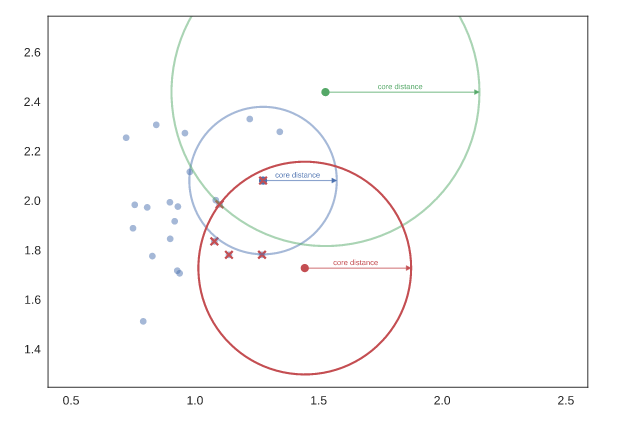
\includegraphics[width=0.5\textwidth]{hdbscan_1}
    \caption{The core distances for three points shown as circles. Source\cite{how_hdbscan_works}}
    \label{fig:hdbscan_1}
\end{figure}

Once the core distances are known, the mutual reachability distance between two points is defined as follows:

\begin{equation*}
    d_{mreach}(a, b) = max\{core_k(a), core_k(b), d(a, b)\}
\end{equation*}

where $d(a, b)$ is the original distance between $a$ and $b$. Therefore if two points are close together, but the density around one point is rather low, the core distance will be greater than the original distance and thus the two points appear to be less close together when considering the mutual reachability distance.

\subparagraph{2. Build the minimum spanning tree}

Based on the mutual reachability distances, the next step is to find points close  to each other. This is done by creating a minimum spanning tree, where edges are weighted according to the mutual reachability distance and a point is represented by a vertex. The minimum spanning tree is created one edge at a time, always choosing the lowest distance to a vertex not yet in the tree. This is done until each vertex is connected, which results in the minimal set of edges, such that dropping any edge will cause the disconnect of one or more vertices from the tree.

\subparagraph{3. Build the cluster hierarchy}

Once the minimum spanning tree is complete, it is converted into a hierarchy of connected clusters, by sorting edges of the tree by distance and iterate through, creating a new merged cluster for each edge. The dendogram in Figure \ref{fig:hdbscan_2} shows a possible cluster hierarchy. %TODO rewrite this paragraph. 

\begin{figure}[h]
    \centering
    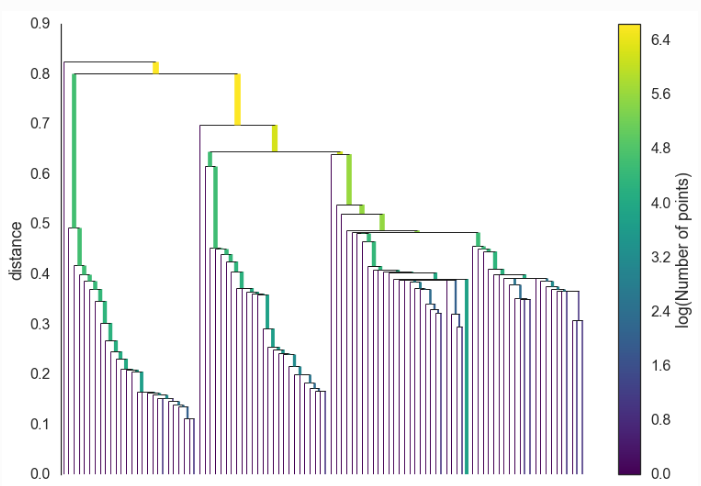
\includegraphics[width=0.5\textwidth]{hdbscan_2}
    \caption{The cluster hierarchy shown as a dendogram. Source\cite{how_hdbscan_works}}
    \label{fig:hdbscan_2}
\end{figure}

At this stage we have to flatten the hierarchy to get the final clusters, which provide the best representation of the current data set. DBSCAN simply cuts through the hierarchy using a fixed parameter, usually called epsilon, to get the final clusters. This approach does not work well with clusters of varying densities and the epsilon parameter itself is unintuitive, requiring further exploration to find optimal values. This is were HDBSCAN improves upon DBSCAN, by taking additional steps for finding relevant clusters.

\subparagraph{4. Condense the cluster tree}

\begin{figure}[h]
    \centering
    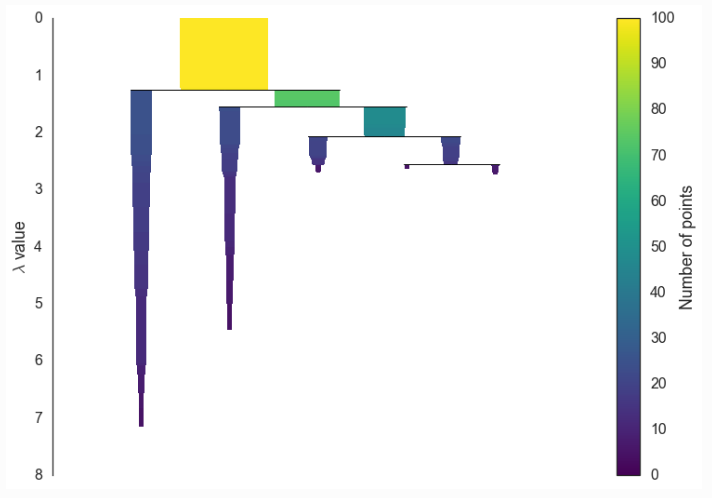
\includegraphics[width=0.5\textwidth]{hdbscan_3}
    \caption{Condensed cluster hierarchy. Source\cite{how_hdbscan_works}}
    \label{fig:hdbscan_3}
\end{figure}

The fourth step consists of condensing the previously built cluster hierarchy into a smaller tree. The process starts at the top where all vertices still belong to the same cluster. Iterating through the hierarchy, for each split the two resulting clusters are compared against a predefined minimum cluster size. If the size of a cluster is below the minimum, its points will be discarded, while the other cluster remains in the parent cluster. If both cluster sizes are above or equal the minimum, the clusters are considered as true clusters. This is repeated until no more splits can be made. 


\subparagraph{5. Extract the clusters}

The extraction of the final clusters from the condensed tree is based on the stability per cluster and once it is selected, none of its subclusters can be chosen. The stability is based on the persistence of a cluster, which is measured by $\lambda = \frac{1}{distance}$. The stability for a cluster $C$ is defined as

\begin{equation}
\sum_{p \in \text{C}}^{|C|} ({\lambda}_{p} - {\lambda}_{birth})
\end{equation}

 where ${\lambda}_{p}$ describes when point $p$ fell out of the cluster and $ {\lambda}_{birth}$ describes when the cluster was created. Now calculating the stability for each cluster starts at the leaf nodes and ends when the root is reached. A cluster is selected if its stability is larger the sum of stabilities of its children. If the sum child stabilities is larger than that of its parent, the parent stability will be set to the value of the sum of its children, but no selection will be done. Based on this approach the final clusters will be selected, with regards to varying densities and noise.
\section{Design and Implementation}

The methodology consist of three parts, where each part builds upon the results from the previous one.
Initially the test data is created, which will be used for all evaluations.
Once the data is available, we evaluate HDBSCAN and determine the settings,
which lead to optimal results regarding our specific use case.
The final part applies the results obtained from the previous evaluation in an online setting.

\subsection{Data flow}
% Todo: Add a box diagram of the data flow
% E.g. News article -> Text preprocessing -> Clustering -> Output


\begin{tikzpicture}[
    squarednode/.style={rectangle, align=center, draw=black!60, very thick, minimum size=5mm},
    ]

    %Nodes
    \node[squarednode] (newsarticle)                                {Collection of\\ news articles};
    \node[squarednode] (preprocessing)  [right=of newsarticle]      {Text preprocessing};
    \node[squarednode] (vectorization)  [right=of preprocessing]    {Vectorization};
    \node[squarednode] (clustering)     [right=of vectorization]    {Clustering};
    \node[squarednode] (result)         [right=of clustering]       {Result};
     
    %Lines
    \draw[->] (newsarticle.east) -- (preprocessing.west);
    \draw[->] (preprocessing.east) -- (vectorization.west);
    \draw[->] (vectorization.east) -- (clustering.west);
    \draw[->] (clustering.east) -- (result.west);

\end{tikzpicture}
    
TODO describe

\subsection{Data Set}
\label{subsec:4a_data_set}

Before any clustering method can be implemented or evaluated,
it is important to rely on the right data set for training and evaluation.

\subsubsection{Data Set Candidates}
\label{subsubsec:4a_data_set_candidates}

As our goal is to detect events in data streams, we have evaluated different data sets and
their possibilities to extract events from their data themselves.

\begin{table}[h]
    \centering
    \begin{tabular}{|l|r|l|}
    \hline
    \textbf{Data set} & \textbf{Number of rows} & \textbf{Description} \\ \hline
    GDELT 2.0 & 575,000,000+ & Print and web news from around the world. \\ \hline
    ChallengeNetwork & 4,449,294 & Network packages including anomalies. \\ \hline
    One Million Posts Corpus & 1,011,773 & User comments to news articles. \\ \hline
    Online Retail Data Set & 541,909 & Customer retail purchases of one year. \\ \hline
    News Aggregator Dataset & 422,937 & Clustered news articles. \\ \hline
    Dodgers Loop Sensor Data Set & 50,400 & Number of cars driven through a ramp. \\ \hline
    10k German News Articles & 10,273 & German news articles. \\ \hline
    \end{tabular}
    \caption{Evaluated data set candidates ordered by data set size.}
    \label{tab:data_set_candidates}
\end{table}

We could extract events from all data sets mentioned in \tabref{tab:data_set_candidates}.\\
The extracted events could be as follows:

\begin{itemize}
    \item Network packages
        \begin{itemize}
            \item Cyber attacks depending on suspicious packets.
        \end{itemize}
    \item User comments
        \begin{itemize}
            \item Change of public opinion during time.
        \end{itemize}
    \item Retail purchases
        \begin{itemize}
            \item Change of purchasing behavior based on product choices.
        \end{itemize}
    \item Traffic
        \begin{itemize}
            \item Traffic changes due to baseball games.
        \end{itemize}
    \item News articles
        \begin{itemize}
            \item Development of a certain news story.
        \end{itemize}
\end{itemize}

However, from above data sets only two contained prelabeled events:

\begin{enumerate}
    \item Dodgers Loop Sensor Data Set
        \begin{itemize}
            \item 81 labeled events. % Todo: x events in y clusters
        \end{itemize}
    \item News Aggregator Dataset
        \begin{itemize}
            \item 422,937 labeled events. % Todo: x events in y clusters
        \end{itemize}
\end{enumerate}

As we did not want to lose too much time in manually clustering data,
we have decided to go with one of these two.
Regarding our two options, our choice was simple:\\
We went for the \textbf{The News Aggregator Dataset} since it not only provided more data,
but our work built on the news articles use case could later be continued with real live data.
The \textbf{GDELT 2.0} data set for example, provides around 1,000 to 2,000 new news articles every 15 minutes.

\subsubsection{Data Retrieval}
\label{subsubsec:4a_data_retrieval}

Unfortunately the data set did not contain the news articles themselves but rather only the URL's to the news articles.
This was done so due to copyright restrictions on the content.
Fortunately there are web scraping tools designed to retrieve the content from news articles specifically.
We decided to use Newspaper3k\cite{newspaper3k},
a Python3 library that allows us to retrieve the text from news articles easily.

The library only requires an URL to download and extract the news article from a website, see following example:

% Todo: Hyphen gets converted inside "lstlisting".
% Copy & paste the URL from the PDF into a browser -> it won't work.
\begin{lstlisting}[language=Python, caption=Retrieve the news article from an URL., label={lst:newspaper3k_code}]
    from newspaper import Article

    url = 'http://fox13now.com/2013/12/30/new-year-new-laws-obamacare-pot-guns-and-drones/'
    article = Article(url)
    article.download()
    article.text # Contains the article's text.
\end{lstlisting}

All we had to do now is to run this code for all news articles.
To speed this process up, we have loaded the data set into a database and run 8 concurrent processes which
retrieved the news articles content from the web in different batches.

\subsubsection{Data Cleansing}
\label{subsubsec:4a_data_cleansing}

The data set contains news articles collected from March 10th to August 10th of 2014.
Five years later, many resources are not online anymore or are not accessible from Europe due to GDPR.
We have used following SQL query to filter out news articles that were most likely corrupt:

\begin{lstlisting}[language=SQL, caption=Retrieve valid news articles., label={lst:valid_news_articles_sql}]
    SELECT *
    FROM news_article
    WHERE
        newspaper_text IS NOT NULL
        AND TRIM(COALESCE(newspaper_text, '')) != ''
        AND hostname NOT IN ('newsledge.com', 'www.newsledge.com')
        AND newspaper_text NOT LIKE '%GDPR%'
        AND newspaper_text NOT LIKE '%javascript%'
        AND newspaper_text NOT LIKE '%404%'
        AND newspaper_text NOT LIKE '%cookie%'
        AND newspaper_keywords NOT LIKE '%GDPR%'
        AND newspaper_keywords NOT LIKE '%javascript%'
        AND newspaper_keywords NOT LIKE '%404%'
        AND newspaper_keywords NOT LIKE '%cookie%'
        AND title_keywords_intersection = 1
\end{lstlisting}

% Todo: Continue cleansing text.

% Todo: The first important step is to create a test data set to run the evaluations with and verify them.
% Todo: explain the source and structrue

% raw text
% with entity extraction
% word embeddings?
% Tfidf

\subsection{Clustering Evaluation}
\label{subsec:4b_clustering_evaluation}

\subsubsection{Design}
\label{subsubsec:4b_design}

The goal of the clustering evaluation is to find the optimal parameters and preprocessing methods for applying HDBSCAN in an online setting.
Therefore the clustering evaluation is designed to run HDBSCAN on our test data,
using a combination of different text processing methods, vector space models and parameters.
\textit{k}-means is used to provide a benchmark for HDBSCAN evaluation.
Once a clustering has been performed, the result is measured based on the ground truth and stored in a database for later analysis.

An important consideration is the variety of samples to use for a clustering run.
Using only a single set of samples might bias the score against this specific set of samples
and some methods might perform better or worse depending on the samples.
To introduce variability, while still retaining repeatability, an evaluation run will be repeated multiple times.
Each repetition will load a new set of sample, iterating linearly through the data set.
For example if we define the number of repetitions as two with a sample size of 1000,
the evaluation will first be done on the first 1000 samples with all possible settings
and the second run will load the next 1000 samples, thus containing sample with indices ranging from 1001 to 2000.
The reason we do not load random sets of samples is repeatability.
If we make any changes in the implementation or the scoring function,
we want to be able to compare the new results with the previous ones in a deterministic manner.

\subsubsection{Scoring Function}
\label{subsubsec:4b_scoring_function}

The scoring function is essential for measuring the result of a clustering method.
The score should reflect the quality of the individual clusters and of the clustering as a whole.
The number of existing measures for clustering is vast and can be split into two main categories.
Internal measures determine the score based on criteria derived from the data itself
and external measures depend on criteria non-existent in the data itself such as class labels.
Since the ground truth is known in our test data, we are going to apply an external measure.

Initially we used Normalized Mutual Information (NMI) as our primary scoring function.
The NMI is an entropy-based measure and tries to quantify the amount shared information between the clusterings.
The score proved to work well for our initial evaluations, but upon closer inspection certain anomalies were found.
An example is given in table \ref{tab:nmi_kmeans_example}, where \textit{k}-means achieved a rather high score,
regardless of the large difference between the true amount of clusters and the approximation using $\sqrt{n}$.
We were not able to explain this behaviour,
although there are multiple papers about the selection bias of NMI for higher numbers of clusters\cite{LEI201758}\cite{clustering_anmi}.
Other scoring functions such as V-Measure or the Adjusted Rand Index showed similar unexpected results with different clusterings.
Therefore we decided to develop our own scoring function based on the ideas of Maximum Matching\cite{data_mining}
and the Jaccard Index, which we call MP-Score.

% TODO add number of estimated clusters
\begin{table}[h]
    \centering
    \begin{tabular}{|l|l|l|l|l|}
    \hline
    \textbf{Algorithm} & \textbf{Sample Size} & \textbf{NMI}  & $\mathbf{n_{true}}$ & $\mathbf{ \mid n_{true} - n_{predicted} \mid }$ \\ \hline
    \textit{k}-means & 19255 & 0.754 & 600 & 457 \\ \hline
    HDBSCAN & 19255 & 0.742 & 600 & 2 \\ \hline
    \end{tabular}
    \caption{\textit{k}-means has a higher NMI score than HDBSCAN, while having a much larger difference in number of clusters.}
    \label{tab:nmi_kmeans_example}
\end{table}

\paragraph{Calculating the score}
The scoring function first calculates the similarity between pairs of clusters,
where each cluster belongs to a different clustering.
We use the Jaccard Index to measure the similarity, which is defined as

\begin{equation}
    \label{equ:similarity}
    \frac{|A \cap B|}{|A \cup B|}
\end{equation}

To illustrate the process we start with an example.
We use $T$ and $C$ as our clusterings, where $T$ is the ground truth and $C$ is the predicted clustering.
The clusterings are defined as follows:

\begin{gather*}
    T = \{\{1,2,3\},\{4,5,6,7\},\{8,9\}\} \\
    C = \{\{1,2\},\{3,4,5,6\},\{7\},\{8,9\}\}
\end{gather*}

We calculate the similarity as defined in Equation \eqref{equ:similarity},
for each possible pair between $T$ and $C$ starting with $t_1= \{1,2,3\}$ and $c_1 = \{1,2\}$:

\begin{align*}
    similarity(t_1,c_1) &=\frac{|t_1 \cap c_1|}{|t_1 \cup c_1|}
    = \frac{|\{1,2\}|}{|\{1,2,3\}|}
    = \frac{2}{3} = 0.667 \\
\end{align*}

After doing this for each possible pair we get the similarity matrix $A$:

\begin{gather*}
\begin{array}{rcl}
    A = & \left(\begin{array}{cccc}
        similarity(t_1,c_1) & \hdots & \hdots & similarity(t_1,c_4)\\
        \vdots & \vdots & \vdots & \vdots\\
        similarity(t_3,c_3) & \hdots & \hdots & similarity(t_3,c_4) \end{array}\right)
        = & \left(\begin{array}{cccc}
            0.667 & 0.167 & 0 & 0 \\
            0 & 0.6 & 0.25 & 0.4 \\
            0 &  0 & 0 & 1.0 \end{array}\right)
\end{array}
\end{gather*}

As a next step we have to select the most relevant similarity values from each row of the similarity matrix.

Finding relevant values in the similarity matrix is non-trivial,
since clusters do not share labels across different clusterings.
To solve this, we make two assumptions based on the principle of Maximum Matching:

\begin{enumerate}
    \item The higher the similarity between two clusters, the more likely it is, that both clusters are describing the same group of documents.
    \item Each cluster can be associated with a cluster from another clustering only once.
\end{enumerate}

Based on those assumptions we select the highest similarity value per row,
whose column is not already associated with another row.
Applying this selection function $f$ to our previously calculated similarity matrix $A$
results in the set containing the most relevant similarity values.

\begin{gather*}
    \begin{array}{rcl}
        f(A) = & \left(\begin{array}{cccc}
            \mathbf{0.667} & 0.167 & 0 & 0 \\
            0 & \mathbf{0.6} & 0.25 & 0.4 \\
            0 &  0 & 0 & \mathbf{1.0} \end{array}\right)
            = \{0.667, 0.6, 1\}
    \end{array}
\end{gather*}

As we can see, there were no collisions between columns and we simply get the highest value per row.
Consider the following example with a different similarity matrix $B$, which does contain a collision:

\begin{gather*}
    \begin{array}{rcl}
        f(B) = & \left(\begin{array}{cccc}
            \mathbf{0.75} & 0.375 & 0.427 & 0.375 \\
            0.4 & \mathbf{0.667} & 0.571 & \textcolor{red}{0.8} \\
            0.333 &  0.25 & 0.4 & \mathbf{1.0} \end{array}\right)
            = \{0.75, 0.667, 1\}
    \end{array}
\end{gather*}

The selected similarity for the second row is 0.667 instead of 0.8.
This is because the fourth column is already associated with the third row, while having an similarity greater than 0.8.
Therefore based on our assumption that clusters cannot be associated twice,
the second highest similarity is used for the second column.
In case no association could be found, the value would be set to zero.

As a third step we have to calculate the weights to be used for the weighted average.
The weight is based on the number of elements inside the cluster
and necessary to represent differences in predicted and true number of clusters in the final score.
It is defined as follows:

\begin{equation}
    \label{equ:weight}
        w_{ij} = \frac{|t_i| + |c_j|}{|T|+|C|} \\
\end{equation}

where $T$ is the ground truth with $t_i \in T$ and $C$ the predicted clustering with  $c_j \in C$.
Therefore the weight for a pairing $t_ic_j$ includes both the size of the true cluster and the size of the predicted cluster.
The reason both sizes are used, is that we want to reflect the difference between the number of predicted clusters and the ground truth.
Using only the true number of elements as the weight, would affect the score if $|C| < |T|$, but not $|C| > |T|$.
Hence the number of predicted elements has to be included into the weight.

To continue our example we have to calculate the weights based on the coordinates of the selected values from our similarity matrix $A$.
The coordinates are $(1,1), (2,2), (3,4)$.
As a result we calculate the following weights:

\begin{align*}
    w_{1,1} &= \frac{|t_1| + |c_1|}{|T|+|C|} = \frac{3 + 2}{9 + 9} = \frac{5}{18} = 0.278 \\
    w_{2,2} &= \frac{|t_2| + |c_2|}{|T|+|C|} = \frac{4 + 4}{9 + 9} = \frac{8}{18} = 0.444 \\
    w_{3,4} &= \frac{|t_3| + |c_4|}{|T|+|C|} = \frac{2 + 2}{9 + 9} = \frac{4}{18} = 0.222
\end{align*}

In the fourth and final step we calculate the weighted average

\begin{equation}
    \label{equ:weighted_average}
        \text{MP-Score} = \sum_{i=0}^{|S|} w_is_i \{w_i \in W \wedge s_i \in S\}
\end{equation}

where $S$ contains the selected values from the similarity matrix with $s_{i} \in S$ and $W$ is the set of weights with $w_i \in W$.
Using our previously selected similarity values $S = f(A) = \{0.667, 0.6, 1\}$
and the corresponding weights $W = \{0.278, 0.444, 0.222\}$,
the calculation for the final average would be done as follows:

\begin{align*}
    \text{MP-Score} = (0.278 \cdot 0.667) + (0.444 \cdot 0.6) + (0.222 \cdot 1) = \mathbf{0.674}
\end{align*}

The final score for the evaluation of the predicted cluster $C$ with the true cluster is 0.674.
The complete implementation of the scoring function can be found in the appendix as Listing \ref{lst:select_max_values}.

\paragraph{Comparison against other measures}
The test scenarios in table \ref{tab:score_scenarios} show the resulting scores of our similarity score, NMI and ARI.
The second scenario results in a ARI score of 0.308, while the NMI with 0.564 and the MP-Score with 0.637 are both higher.
Intuitively we would assume the higher score to better represent the predicted clustering,
since the number of clusters is correct and only two out of nine elements are assigned to the wrong cluster.
Scenario six shows a similar case.
Scenarios four and especially five show the previously mentioned bias of NMI with regards to higher numbers of clusters.
The seventh scenario gives an interesting result were both NMI and ARI result in zero while the MP-Score results in 0.321.
The relatively high MP-Score is because a true cluster with four elements is matched with the predicted cluster containing nine elements.
This result in a similarity of 0.444, which is then lowered by the weight.
The NMI does not infer any entropy, since every element ends up in the same cluster independently from the ground truth.
The ARI results in zero because of its adjustment for chance.
Overall the MP-Score behaves rather intuitively, although it is not corrected for randomness.
This means even a completely random clustering would result in a MP-Score greater than 0,
while an adjusted measure such as the ARI would be 0 in such a case.

\begin{table}[h]
    \centering
    \begin{tabular}{|l|l|l|l|l|}
    \hline
    \multicolumn{5}{ |c| }{\textbf{Test scenarios with ground truth $T = \{\{1,2,3\},\{4,5,6,7\},\{8,9\}\}$}} \\
    \hline
    Nr. & Predicted Clustering $C$ & NMI & ARI & MP-Score \\ \hline
    1 & $C = \{\{1,2,3\},\{4,5,6,7\},\{8,9\}\}$ & 1.0 & 1.0 & 1.0 \\ \hline
    2 & $C = \{\{1,2\},\{3,4,5,6\},\{7,8,9\}\}$ & 0.564 &  0.308 & 0.637 \\ \hline
    3 & $C = \{\{1,2,3\},\{4,5,6\},\{7\},\{8,9\}\}$ & 0.895 & 0.771 & 0.847 \\ \hline
    4 & $C = \{\{1,2,3\},\{4,5\},\{6,7\},\{8\},\{9\}\}$ & 0.821 & 0.591 & 0.583 \\ \hline
    5 & $C = \{\{1\},\{2\},\{3\},\{4\},\{5\},\{6\},\{7\},\{8\},\{9\}\}$ & 0.651 & 0 & 0.227 \\ \hline
    6 & $C = \{\{1,2,3,4,5\},\{6,7,8,9\}\}$ & 0.434 & 0.182 & 0.433 \\ \hline
    7 & $C = \{\{1,2,3,4,5,6,7,8,9\}\}$ & 0.0 & 0 & 0.321 \\ \hline
    8 & $C = \{\{7,2,4\},\{8,9,6,3\},\{1,5\}\}$ & 0.219 & -0.108 & 0.392 \\ \hline
    \end{tabular}
    \caption{Direct comparison of different scoring functions}
    \label{tab:score_scenarios}
\end{table}

As a final note, repeating the evaluation shown in table \ref{tab:nmi_kmeans_example} a second time using the MP-Score,
the score (Table \ref{tab:avg_predict_kmeans_example}) for \textit{k}-means is much lower than HDBSCAN.
This reflects what we would expect based on the big difference in the amount of predicted clusters.

\begin{table}[h]
    \centering
    \begin{tabular}{|l|l|l|l|l|}
    \hline
    \textbf{Algorithm} & \textbf{Sample Size} & \textbf{Similarity}  & $\mathbf{n_{true}}$ & $\mathbf{ \mid n_{true} - n_{predicted} \mid }$ \\ \hline
    \textit{k}-means & 19255 & 0.137 & 600 & 457 \\ \hline
    HDBSCAN & 19255 & 0.605 & 600 & 2 \\ \hline
    \end{tabular}
    \caption{The similarity score reflects the difference in number of predicted clusters.}
    \label{tab:avg_predict_kmeans_example}
\end{table}

\subsubsection{Implementation}
\label{subsubsec:4b_implementation}

The evaluation process is done with our own evaluation framework.
The framework allows for automated and repeatable evaluation runs.
Results are stored in a database for later analysis.
The main features include:

\begin{itemize}
    \item Defining the number of stories to run the evaluation with and load all news articles from those stories.
    \item Repeating evaluation runs with different sets of data.
    \item Providing different vector space models for converting the textual data into a vector space model.
    \item Defining a range for each parameter of a clustering method and running it with each possible combination of those parameters.
    \item Storing the result the result in a database and creating relations between news articles, clusters and evaluation runs. This allows for manual inspection and analysis of individual articles inside a predicted cluster.
\end{itemize}

The implementation is done with Python.
Clustering methods and vector space models are provided by the scikit-learn library\cite{scikit-learn},
while the specific HDBSCAN implementation is provided by a scikit-learn-contrib package\cite{McInnes2017}.
scikit-learn-contrib is a collection of high quality third-party projects compatible with scikit-learn.
We decided to use scikit-learn because of its rich documentation,
the wide range of tools and algorithms it provides for clustering and our previous experience with it.
Additionally the framework runs in a fully dockerized environment, which includes the database.
This allows the framework to run independently from the underlying host, as long as the host supports docker.
This principle was useful for developing and testing the framework in a local environment and deploying it on a remote server for long running evaluations,
without worrying about setting up and installing all dependencies again.

\paragraph{Defining cluster parameters}
The parameters for each available clustering method are defined beforehand in a dictionary as can be seen in Listing \ref{lst:cluster_method_parameters}.
Parameters are defined as a list of possible variations.
For example if we want to run HDBSCAN with two different metrics \textit{cosine} and \textit{euclidean},
we define the metric parameter as \lstinline{"metric": ["cosine", "euclidean"]}.
When running a clustering method, it will be executed with each possible combination of parameters.
This means a single evaluation of HDBSCAN, will include 16 different runs,
since there are two different metrics and eight different options for $min\_cluster\_size$.
This is important to consider for running clustering methods with long processing times or running evaluations on large sample sizes.

\begin{lstlisting}[caption=Predefined parameters for different clustering methods,label={lst:cluster_method_parameters}]
parameters_by_method = {
    self.kmeans: {
        "n_cluster": ["n_square", "n_true"]
    },
    self.hdbscan: {
        "min_cluster_size": range(2, 10),
        "metric": ["cosine", "euclidean"]
    },
    self.meanshift: {"cluster_all": [True, False]},
    self.birch: {
        "branching_factor": range(10, 100, 10),
        "threshold": range(2, 6),
    },
    self.affinity_propagation: {
        "affinity": ["euclidean"],
        "convergence_iter": [15],
        "damping": np.arange(0.5, 0.9, 0.1),
        "max_iter": [50, 100, 200, 500],
    },
    self.spectral_clustering: {
        "affinity": ["rbf"],
        "assign_labels": ["kmeans", "discretize"],
    },
}
\end{lstlisting}

\paragraph{CLI}
The evaluation framework provides a command line interface to start evaluation runs and specify a number of settings.
Listing \ref{lst:cluster_evaluation_framework} shows the full interface.

\begin{lstlisting}[caption=Command line interface for the evaluation framework, label={lst:cluster_evaluation_framework}]
usage: cluster_evaluation_framework.py [-h] [--rows ROWS] [--stories STORIES]
                                       [--methods METHODS]
                                       [--vectorizers VECTORIZERS]
                                       [--tokenizers TOKENIZERS] [--runs RUNS]

Run different clustering methods, with a variety of different settings.
data_mining
optional arguments:
  -h, --help            show this help message and exit
  --rows ROWS           number of samples to use for clustering 
                        default: 1000
  --stories STORIES     number of stories to load samples from. This parameter overrides the rows parameter if set.
  --methods METHODS     options: kmeans, hdbscan, meanshift, birch, affinity_propagation, spectral_clustering 
                        default: all available options
  --vectorizers VECTORIZERS
                        options: CountVectorizer, TfidfVectorizer 
                        default: all available options
  --tokenizers TOKENIZERS
                        options: newspaper_text, text_keyterms, text_entities, text_keyterms_and_entities, text_lemmatized_without_stopwords, text_stemmed_without_stopwords 
                        default: all available options
  --runs RUNS           number of runs per clustering method 
                        default: 1
\end{lstlisting}


% TODO write it better

\subsection{Online Clustering}
\label{subsec:4c_online_clustering}

\subsubsection{Design}
\label{subsubsec:4c_design}

Detecting events in a stream of news articles will be achieved by using an online clustering approach.
An event is described by the occurrence of multiple news articles about the same story.
The events of interest for this application are the discovery of new stories and the extension of existing stories.
Thus we define our two types of events as follows:

\begin{itemize}
    \item New event: A new cluster of news articles appears in the data stream, which describe the same story.
    \item Event extended: An existing story is extended by additional news articles.
\end{itemize}

HDBSCAN will be applied as the clustering method,
using the optimal settings discovered in the clustering method evaluation.
Additional preprocessing of news articles before clustering is going to be explored
as part of evaluation as well and will be implemented accordingly for the online clustering.

The clustering will be done in batches over time, since HDBSCAN only supports static data sets.
Events are detected by comparing clusters from successive batches.
\figref{fig:timeline} illustrates this with three batches,
where the resulting clusters from batch $t$ will be compared with the previous result from batch $t - 1$,
while batch $t - 1$ was previously compared with batch $t - 2$.
In this example each batch only contains samples from a limited time period,
where $\triangle t$ stands for the time period between batches.
Since a batch does not contain the full set of samples, we have to consider the overlap between batches.
The size of the overlap is essential to find similar clusters from different batches.
If a similar cluster already exists in the previous batch
the differences between these clusters are detected as a change in an existing event.
If no pair exists for a cluster from a current batch, this cluster will be regarded as a new event.
The similarity between clusters is based on the same assumptions
as for the scoring function described in \subsubsecref{subsubsec:4b_scoring_function}.

\begin{figure}[h]
    \centering

    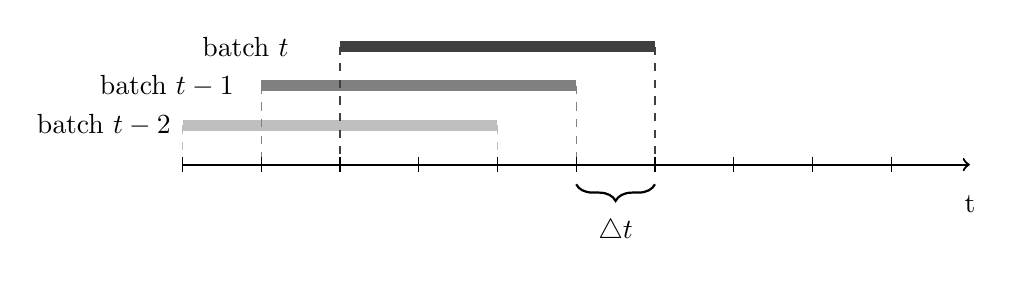
\begin{tikzpicture}[scale=1]

        \draw[lightgray, line width=4pt] (0,.5) -- (4,.5);
        \draw[lightgray, dashed] (0,.5) -- (0,0);
        \draw[lightgray, dashed] (4,.5) -- (4,0);
        \node[align=right] at (-1,.5) {batch $t - 2$};

        \draw[gray, line width=4pt] (1,1) -- (5,1);
        \draw[gray, dashed] (1,1) -- (1,0);
        \draw[gray, dashed] (5,1) -- (5,0);
        \node[align=right] at (-.2,1) {batch $t - 1$};

        \draw[darkgray, line width=4pt] (2,1.5) -- (6,1.5);
        \draw[darkgray, dashed] (2,1.5) -- (2,0);
        \draw[darkgray, dashed] (6,1.5) -- (6,0);
        \node[align=right] at (0.8,1.5) {batch $t$};

        \node[align=center] at (5.5,-0.85) {$\triangle t$};
        \node[align=center] at (10,-0.5) {t};

        \draw [thick,->] (0,0) -- (10,0);
        \foreach \x in {0,...,9} \draw (\x,0.1) -- (\x,-0.1);

        \draw [thick,decorate,decoration={brace,amplitude=6pt,raise=0pt,mirror}] (5,-0.25) -- (6,-0.25);

        \end{tikzpicture}

    \caption{Timeline showing the sliding window approach.}
    \label{fig:timeline}
\end{figure}

The overlap between batches depends on the batch size and the number of new samples in $\triangle t$.
A high volume of incoming samples combined with a small batch sizes
would result in an overlap too small to find pairs of clusters.
All clusters from the current batch would be detected as new in such a case.
To decrease the negative impact on the event detection by peaks in the data stream,
we need a batch size which grows accordingly.
The ideal batch size therefore provides enough overlap between batches to find pairs of clusters
and small enough to allow for efficient processing.
We explore three different methods for determining the ideal batch size:

\begin{enumerate}
    \item \textbf{Fixed size}: The first method uses a fixed batch size,
          where each batch processes the most recent \textit{n} samples.
          This makes the clustering unstable against sudden peaks in the volume of incoming data,
          but we consider this method as an useful benchmark for the dynamic methods.
    \item \textbf{Size by hours}: This method uses a dynamic batch size
          by loading the samples from the last \textit{n} hours.
          This enables the batch size to increase and decrease with the volume of the data stream.
          The number of samples will be limited by an upper bound,
          to keep the space and time consumption of the clustering method reasonable.
    \item \textbf{Size by incoming data}: This method defines the batch size relative to the incoming stream of data.
          We count the number of new samples since the last batch and multiply it by a predefined factor.
          For example if we want the new samples to be 1\%
          of the overall clustering, we define the factor as 100.
          The batch size will be limited by a lower and an upper bound.
          The lower bound prevents the overlap between batches from getting too small.
          The upper bound is based on the same reasoning as mentioned in the previous method.
\end{enumerate}

The evaluation will use the MP-Score to measure the precision of the event detection,
since our model represents events as a clusters.
True events can be extracted directly from the ground truth based on news articles from two successive batches.

\subsubsection{Implementation}
\label{subsubsec:4c_implementation}

The online clustering implemented for this thesis does not operate in a true online setting,
but rather it takes our existing test data and simulates a data stream over time.
The simulated approach allows us to directly compare the resulting events
with the ground truth and thus evaluate different settings.
The implementation is done with Python and runs in a dockerized environment similar to the evaluation framework.

The detection of events relies on comparing clusters between successive batches. 
We apply \gls{lsh}\cite{alex2015practical} to find clusters most similar to each other.
In its essence \gls{lsh} is an efficient way to find similar documents, 
which does not require to calculate the similarity between each possible pair of documents. 
The implementation for \gls{lsh} is provided by the datasketch library\cite{eric_zhu_2017_290602}.

Once we have found pairs of clusters, which represent the same story, detecting events becomes trivial.
For each pair we subtract the current cluster with the cluster from the previous batch. 
The resulting set contains all news articles, which are only present in the current cluster.
These articles are then summarized as a change of an existing event. 
If the previous batch did not contain any similar clusters for a cluster from the current batch, 
the cluster is considered as a new event.

Since events are themselves clusters of news articles,
we apply the MP-Score to measure the precision of detected events. 
Calculating the score is $O(n^2)$, but since the application runs on a simulated timeline and the scoring is only part of the evaluation,
time complexity is a minor concern in this case.

\paragraph{CLI}
The application provides a command line interface to run the simulation with different parameters
such as the start date, number of days to run and the batch size.

\begin{lstlisting}[caption=Command line interface for the online clustering., label={lst:cli_online_clustering}]
usage: online_clustering.py [-h] [--verbose] [--persist_in_db] 
                            [--rows ROWS] [--hours HOURS] 
                            [--factors FACTORS] --date DATE
                            [--run_n_days RUN_N_DAYS] 
                            [--threshold THRESHOLD]

Run the batchwise clustering over a simulated stream of news articles.

optional arguments:
-h, --help              show this help message and exit
--verbose               default: False
--persist_in_db         default: False
--rows ROWS             numbers of samples to process per batch
--hours HOURS           numbers of hours to load samples
--factors FACTORS       factor to use for relative batch sizes
--date DATE             start date
--run_n_days RUN_N_DAYS number of days to run the batchwise clustering
                        default: 1
--threshold THRESHOLD   similarity threshold for cluster matching
                        default: 0.75

\end{lstlisting}


\section{Results}

\subsection{Clustering Evaluation}

The goal of this evaluation is to measure the accuracy of HDBSCAN, with different parameters and preprocessing methods. The most suitable approach will then be used for the online clustering to detect changes in a news stream.

\subsubsection{Setup}

\paragraph{Text Preprocessing}

 The first step in working with text is to apply Natural Language Processing techniques for improving the quality of the data before clustering it. We look the five different preprocessing methods  as described in section \ref{} and evaluate each. The methods are:
 \begin{itemize}
     \item Full text with stop word removal
     \item Key terms
     \item Named Entities
     \item Text Lemmatisation
     \item Text Stemming
 \end{itemize} 

\paragraph{Text Vectorization} Before the text can be clustered, it has to be transformed into a vector space model. We look at two different models:
\begin{itemize}
    \item Word Frequency
    \item tf-idf
\end{itemize}

\paragraph{Parameters} HDBSCAN has a range of parameters, which can be tuned to fit our data set. We focus on the two primary ones:
\begin{itemize}
    \item Min cluster size: The minimum size of a cluster. We run the evaluation with a range from two to nine as the $min\_cluster\_size$. 
    \item Metric: The distance measure between points. We apply the metrics "cosine" and "euclidean". 
    
\end{itemize}

The primary parameter for K-Means is the number of clusters. Since K-Means is used as a baseline to evaluate HDBSCAN, we provide the true number of clusters for each run. Therefore K-Means runs with an optimal starting point. 

\paragraph{Running the evaluation} The evaluation is done with different sets of news articles per run. This means if we define a run to use 30 stories and set it to repeat five times, each repeat will load 30 different stories from the data set. This is done to get a more diverse set of samples. Each run will be repeated at least three times. Lower numbers of stories allow for more repetitions due to lower processing times.   

\subsubsection{Evaluation}

The first run is done with 60 stories, which results in approximately 2000 news articles, over five repetitions. Table \ref{tab:cluster_parameters} shows the resulting accuracy for each parameter in combination with each preprocessing method and vector space model. The highest score per parameter is highlighted as bold. The first insight we get is the variety in accuracy scores for different min cluster sizes. The lowest min cluster size results in the lowest accuracy, while increasing this parameter leads to an increasingly better score. The highest accuracy is reached with a min cluster size of six, while increasing it further reduces the score again. The large difference in accuracy between different min cluster sizes, shows the importance this parameters has on the quality of the clustering and requires some knowledge of the data beforehand. In our case we have a wide range of different cluster sizes as shown in Figure \ref{fig:articles_per_story_distribution}, with clusters containing as little as two news articles. Based on this distribution we expected the min size cluster size to be low. The distribution also explains the drop in accuracy after a min cluster size of 6, since an increasingly number of clusters are being ignored.

\begin{table}[h]
    \centering
    \scalebox{0.65}{
    \begin{tabular}{|l|rrrrr|rrrrr|}
        \hline
        \textbf{Clustering} & \multicolumn{5}{ |c| }{\textbf{Word Frequency}} & \multicolumn{5}{ |c| }{\textbf{tf-idf}} \\
        \hline
        \textbf{HDBSCAN} & Full Text &  Key terms & Entities & Lemmatised & Stemmed & Full Text & Key terms & Entities & Lemmatised & Stemmed \\
        \hline
        min\_size: 2, metric: cosine    & 0.289 & 0.265 & 0.223 & \textbf{0.305} & 0.297 & 0.286     & 0.268 & 0.26      & 0.296     & 0.3       \\
        min\_size: 2, metric: euclidean & 0.101 & 0.093 & 0.110 & 0.101     & 0.106 & 0.301     & 0.170 & 0.241     & \textbf{0.306} & 0.301     \\
        min\_size: 3, metric: cosine    & 0.488 & 0.456 & 0.465 & 0.48      & 0.487 & 0.472     & 0.446 & 0.457     & \textbf{0.493} & 0.478     \\
        min\_size: 3, metric: euclidean & 0.172 & 0.129 & 0.176 & 0.174     & 0.182 & 0.472     & 0.306 & 0.464     & \textbf{0.500} & 0.478     \\
        min\_size: 4, metric: cosine    & 0.630 & 0.555 & 0.625 & 0.552     & 0.577 & 0.577     & 0.586 & \textbf{0.646} & 0.589     & 0.581     \\
        min\_size: 4, metric: euclidean & 0.320 & 0.182 & 0.214 & 0.315     & 0.332 & 0.611     & 0.416 & 0.559     & 0.613     & \textbf{0.615} \\
        min\_size: 5, metric: cosine    & 0.716 & 0.652 & 0.656 & \textbf{0.718} & 0.718 & 0.688     & 0.664 & 0.632     & 0.686     & 0.692     \\
        min\_size: 5, metric: euclidean & 0.355 & 0.217 & 0.266 & 0.41      & 0.389 & \textbf{0.703} & 0.512 & 0.607     & 0.686     & 0.692     \\
        min\_size: 6, metric: cosine    & 0.693 & 0.715 & 0.608 & 0.701     & 0.708 & 0.738     & 0.729 & 0.613     & \textbf{0.751} & 0.747     \\
        min\_size: 6, metric: euclidean & 0.179 & 0.280 & 0.292 & 0.202     & 0.164 & 0.738     & 0.408 & 0.622     & \textbf{0.778} & 0.763     \\
        min\_size: 7, metric: cosine    & 0.631 & 0.611 & 0.552 & 0.643     & 0.634 & 0.689     & 0.685 & 0.553     & 0.718     & \textbf{0.722} \\
        min\_size: 7, metric: euclidean & 0.122 & 0.392 & 0.307 & 0.073     & 0.099 & 0.689     & 0.336 & 0.539     & 0.718     & \textbf{0.722} \\
        min\_size: 8, metric: cosine    & 0.571 & 0.603 & 0.514 & 0.592     & 0.574 & 0.685     & 0.647 & 0.531     & \textbf{0.711} & 0.695     \\
        min\_size: 8, metric: euclidean & 0.056 & 0.339 & 0.338 & 0.025     & 0.057 & 0.685     & 0.286 & 0.522     & \textbf{0.711} & 0.695     \\
        min\_size: 9, metric: cosine    & 0.542 & 0.569 & 0.476 & 0.544     & 0.541 & 0.602     & 0.614 & 0.499     & 0.637     & \textbf{0.640} \\
        min\_size: 9, metric: euclidean & 0.065 & 0.236 & 0.310 & 0.025     & 0.033 & 0.602     & 0.216 & 0.475     & 0.637     & \textbf{0.640} \\
        \hline
        \textbf{K-Means} & \multicolumn{5}{ |c| }{}  & \multicolumn{5}{ |c| }{} \\
        \hline
        n\_cluster: n\_true              & 0.531 & 0.588 & 0.514 & 0.536     & 0.536 & \textbf{0.713} & 0.653 & 0.584     & 0.672     & 0.693     \\
        \hline
    
    \end{tabular}   
    }
    \caption{Accuracy for combinations of parameter and preprocessing with a sample size of 60 stories (approx. 2000 articles)}
    \label{tab:cluster_parameters}
\end{table}

Comparing the two vector models, shows the majority of best scores per parameter achieved by tf-idf. Additionally the different metrics show a significant difference when using the vector model based on word count. With tf-idf the difference between both metrics is often negligible.

As for the optimal preprocessing, text lemmatisation appears to provide the highest accuracy in general
or at least being fairly close to the highest score.
This is to be expected, since text lemmatisation reduces the dimensions by grouping words into their base form,
while still retaining most of the text.
In contrast to key term and entity extraction, which both result in a drastic reduction of the dimensions,
and therefore less detail.
It is important to note, that we used pretrained models for key term and entity extraction.
Specifically training on a news corpus might improve the performance of both methods,
but it was decided as to be out of scope for this thesis.

\begin{figure}[h]
    \centering
    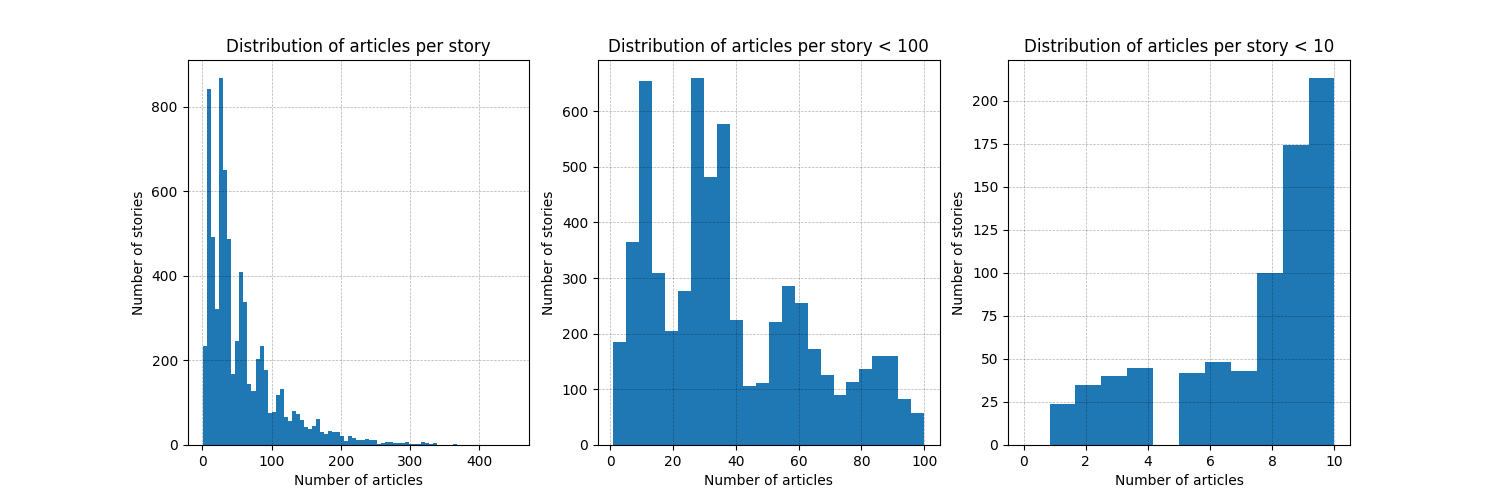
\includegraphics[width=1\textwidth]{articles_per_story_distribution}
    \caption{Distribution of cluster sizes.}
    \label{fig:articles_per_story_distribution}
\end{figure}

After determining the optimal settings for text preprocessing and vectorization, we increase the sample sizes for our evaluation runs, to get a deeper insight into the behaviour of HDBSCAN with larger data sets. Figure \ref{fig:hdbscan_parameters} shows the scores achieved with different parameters over an increasingly large set of samples. Based on this Figure we see the metric $cosine$ to be generally better than $euclidean$, even if $euclidean$ is occasionally more accurate.

% TODO explain why cosine is generally better than euclidean
% TODO explain min cluster sizes, but run with lemmatization

\begin{figure}[h]
    \centering
    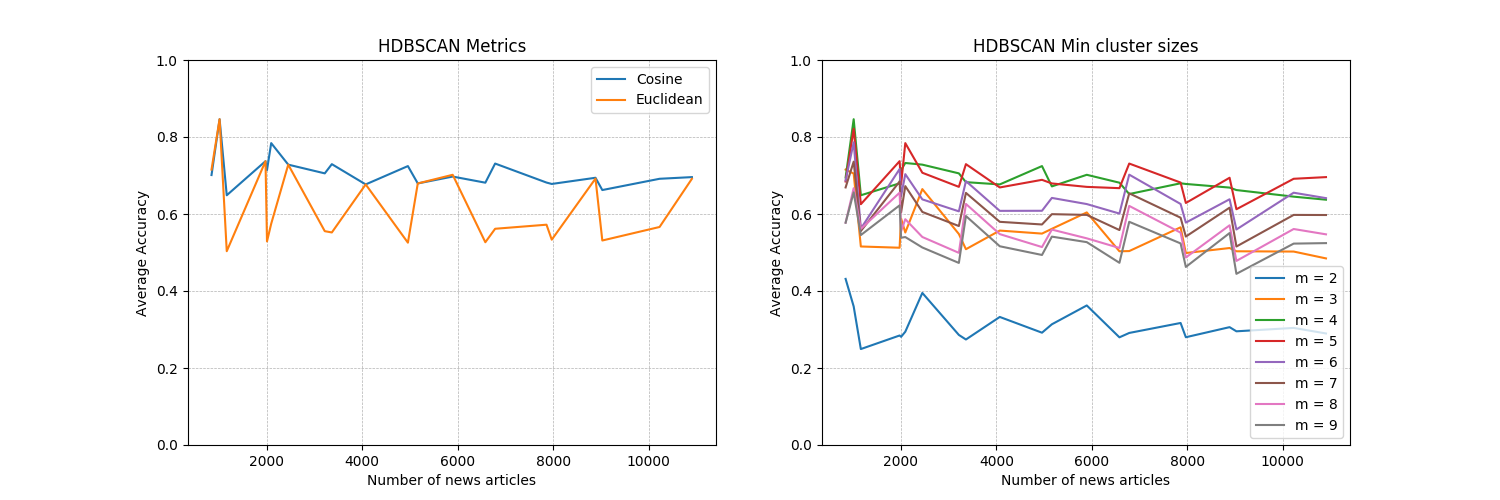
\includegraphics[width=1\textwidth]{hdbscan_parameters}
    \caption{Accuracy for different parameters}
    \label{fig:hdbscan_parameters}
\end{figure}

One of the advantages HDBSCAN has over other clustering algorithms, is the ability to work with noise, since we intent on applying it in an online setting, where noisy data is to be expected. At the same time, the number of articles classified as noise should be kept to a minimum. However the noise ratio shown in Figure \ref{fig:noise_ratio_samples} is higher, than we would expect it to be based on our test data. A variety of factors play into the high noise ratio. One major influence is due to the used $min\_cluster\_size$. Each news article belonging to a cluster ignored due to a size too small, will be counted as noise. In addition to the false positives due to the min cluster size, the test data does still contain noisy data, even after our efforts in cleaning up the data as good as possible. Nonetheless the expected noise ratio based on the test data is less than 10\%, nowhere close to the 20\% of the current evaluation. Decreasing the noise ratio is certainly an important part in future improvements.

% TODO calculate expected noise ratio based our min cluster sizes.

% experiment with min_samples

\begin{figure}[h]
    \centering
    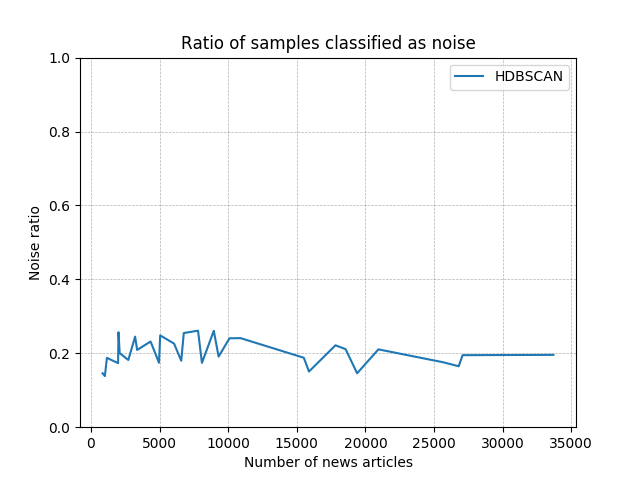
\includegraphics[width=0.5\textwidth]{noise_ratio_samples}
    \caption{Number of news articles classified as noise.}
    \label{fig:noise_ratio_samples}
\end{figure}


Having found the optimal settings to run HDBSCAN with, we can start comparing the overall performance with K-Means. Figure \ref{fig:accuracy_kmeans_hdbscan} shows  a similar behaviour for both clustering methods in value and variance of the accuracy. Although HDBSCAN is generally more accurate than K-Means, the difference gets smaller with an increase in the sample size. 

Increasing the sample size results for both HDBSCAN and K-means in a small loss regarding the accuracy as can be seen in Figure \ref{fig:accuracy_kmeans_hdbscan}. However the accuracy seems to stabilize around the 0.7 mark.

\begin{figure}[h]
    \centering
    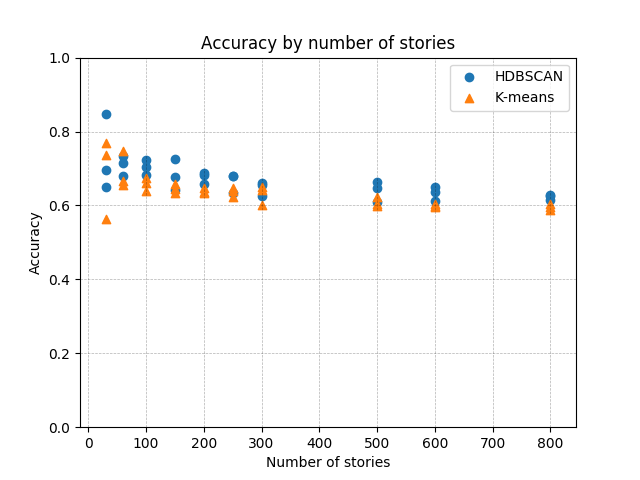
\includegraphics[width=0.5\textwidth]{accuracy_kmeans_hdbscan}
    \caption{Comparison of the average accuracy between K-means and HDBSCAN}
    \label{fig:accuracy_kmeans_hdbscan}
\end{figure}

While HDBSCAN and K-means provide a similar accuracy, the biggest difference can be noted in the processing time in relation to the number of samples. K-means has a time complexity of $O(n^2)$ in contrast to HDBSCAN with a time complexity of $O(nlog(n))$, which is demonstrated by Figure \ref{fig:processing_time_kmeans_hdbscan}. Although running the evaluation has also shown the space complexity for HDBSCAN to be substantially higher for larger amounts of samples than with K-means. Trying to run HDBSCAN with 100'000 news articles caused in a memory error, even with 64GB of RAM, while K-means was able to complete the clustering.

% TODO measure memory?

\begin{figure}[h]
    \centering
    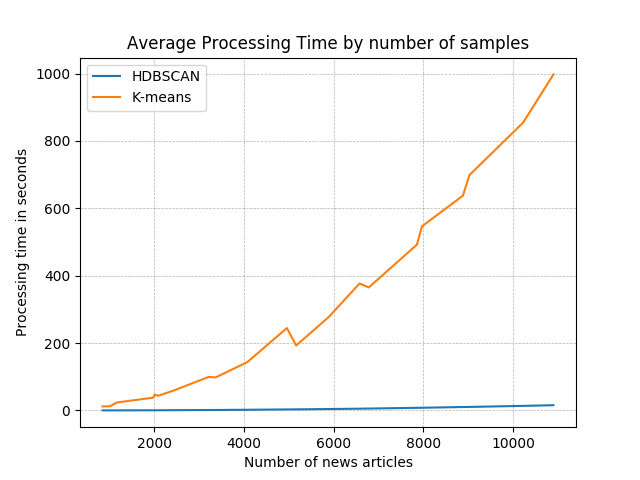
\includegraphics[width=0.5\textwidth]{processing_time_kmeans_hdbscan}
    \caption{Processing time in seconds }
    \label{fig:processing_time_kmeans_hdbscan}
\end{figure}

Figure \ref{fig:cluster_difference_samples} shows, that the difference between predicted over the true number of clusters is fairly low and appears to be roughly linear with the overall number of clusters.  

\begin{figure}[h]
    \centering
    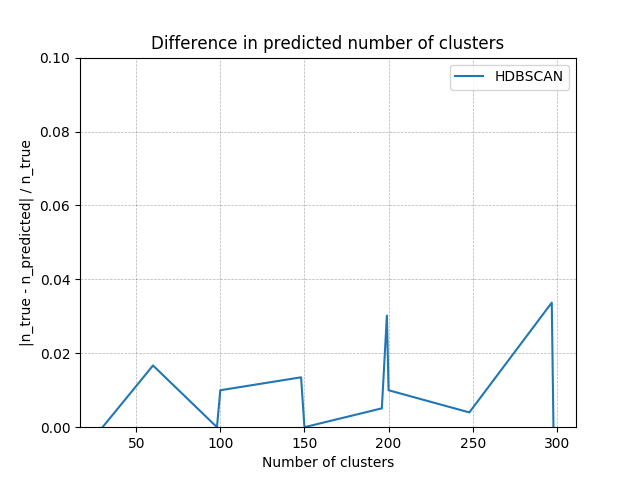
\includegraphics[width=0.5\textwidth]{cluster_difference_samples}
    \caption{Ratio of difference over predicted with true number of clusters}
    \label{fig:cluster_difference_samples}
\end{figure}

As a final note, we compare HDBSCAN with six different clustering methods taken from scikit-learn. Each method is run with a variety of parameters and the best scores are shown in Figure \ref{fig:different_clusterings}. HDBSCAN provides the highest accuracy, while being still being one of the fastest algorithms. Based on this data, we can assume HDBSCAN to be a good candidate for our use case.

\begin{figure}[h]
    \centering
    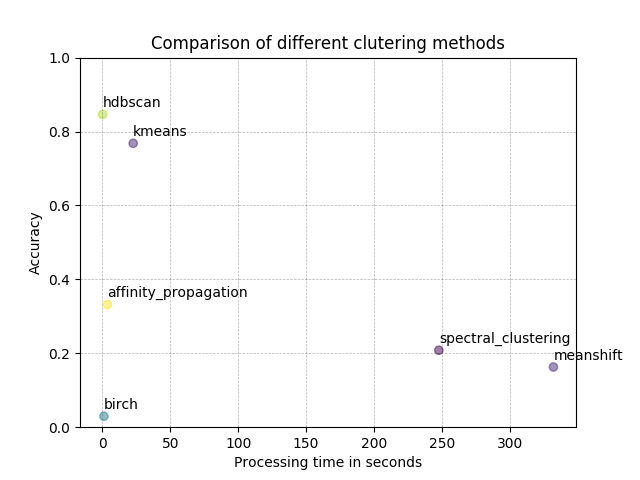
\includegraphics[width=0.5\textwidth]{different_clusterings}
    \caption{Comparison of different clustering methods with a sample size of approximately 1000 news articles}
    \label{fig:different_clusterings}
\end{figure}

\subsubsection{Conclusion}

% TODO: This conclusion belongs to the chapter "Conclusion"
The evaluation has shown HDBSCAN to be a good candidate to use for news clustering. It provides an better accuracy than K-means, while being significantly faster to process. The predicted number of clusters is consistent with an increasing number of samples and fairly close the truth. Additionally we have shown the required preprocessing and vectorization steps with the ideal parameters to achieve the most accurate results for our data set. On the flip side the noise ratio is quite high and the space complexity is problematic with larger data sets. Overall HDBSCAN provides an acceptable accuracy, while still leaving room for further improvements.

\subsection{Online clustering}

\subsubsection{Setup}

The online clustering is done on a simulated stream of news articles based on the same data set as used in the clustering evaluation. This allows for direct comparison between the detected events and the ground truth. The settings to run the clustering are as follows:

\begin{itemize}
    \item Text Lemmatisation
    \item Vectorizer: tf-idf
    \item Clustering method: HDBSCAN
    \item Min cluster size: 5
    \item Distance metric: cosine
\end{itemize}

The clustering is run over 30 days with a total of 42'916 news articles. The distribution of news articles this time period is illustrated in Figure \ref{fig:news_articles_over_time}.

\begin{figure}[h]
    \centering
    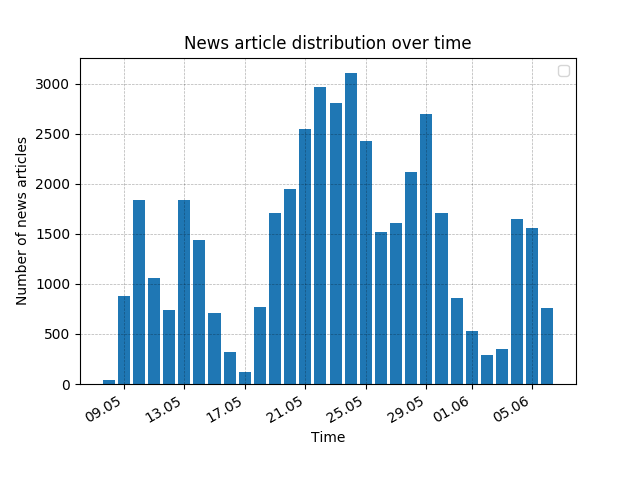
\includegraphics[width=0.5\textwidth]{news_articles_over_time}
    \caption{Incoming news articles over 30 days}
    \label{fig:news_articles_over_time}
\end{figure}

\subsubsection{Evaluation}

The goal of the online clustering is to detect new events in an incoming stream of news articles and changes in existing events. This evaluation analyses the results of our simulated test runs with different batch sizes.

Figure \ref{fig:event_detection_differences} shows the differences between the number of detected events and the number of true events for both new and existing topics. Based on this data we see the impact of different batch sizes for the accuracy in detected events. The difference with a batch size of 5000 news articles is significantly lower than the batch size of 1000. The difference is especially noticeable in the time period between the 21.05 and 25.05. The reason for this spike can be found in the distribution of incoming news articles as shown in Figure \ref{fig:news_articles_over_time}. During this period we receive up to 3000 news articles in a single day. This means by using a lower batch size such as 1000, the overlap between batches gets too small to reliably detect changes between batches, which causes too many new topics to be detected. 

\begin{figure}[h]
    \centering
    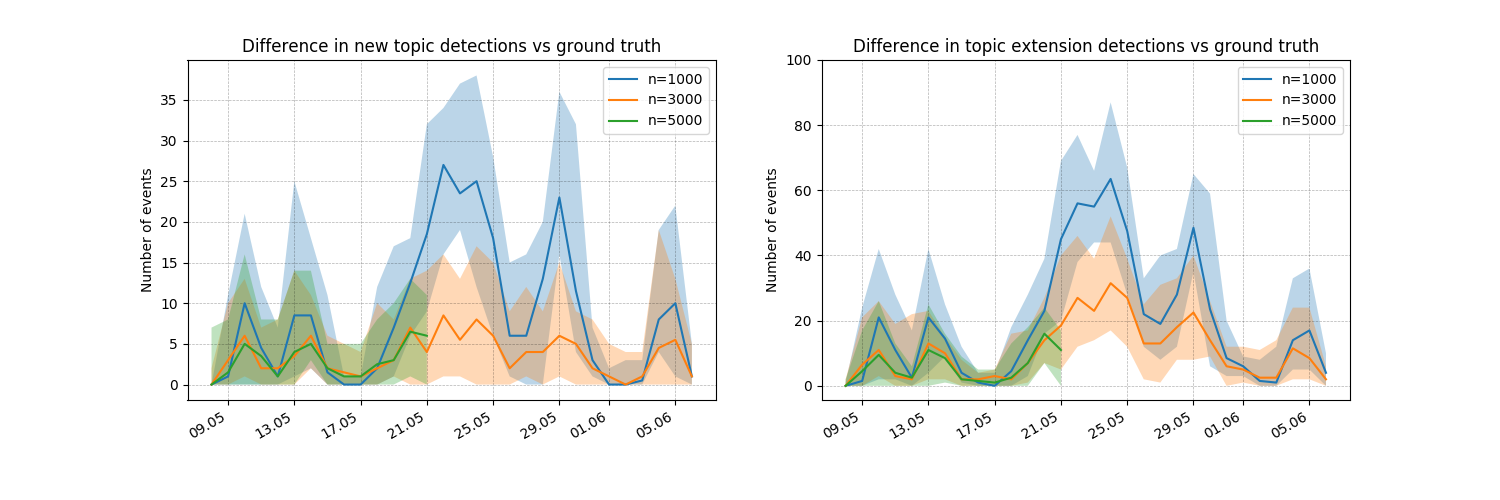
\includegraphics[width=1\textwidth]{event_detection_differences}
    \caption{Comparison between the difference in detected and true events}
    \label{fig:event_detection_differences}
\end{figure}

Although a larger batch size does not simply equal a better difference, as can be seen in Figure \ref{fig:event_detection_differences} by comparing the differences using a batch size of 3000 with a batch size of 5000. The batch size n=3000 shows a generally lower difference in the detection of new events than with n=5000. The differences between both batch sizes are less significant when detecting changes in existing events.

Based on the overall differences, we do not know the accuracy of those predictions. If the difference between newly detected events and true events is zero, there is still the possibility, that the events itself are different from the ground truth, and thus contain false positives. To measure the quality of events, we can look at the collection of events in a single batch as a subset of clusters, where each event is represented by a cluster containing all relevant news articles. Since we now have two clusterings, one containing detected events and the other with events taken from the ground truth, we can apply our MP-Score as a metric to get an insight into the quality of the detected events over the ground truth. Figure \ref{fig:event_detection_mp_score_1000} shows the MP-Scores for an online clustering using a batch size of 1000. Since there is quite a large variance, the score is shown as a boxplot, where a single box represents a full day. The large variance is already the first indication, that the quality is rather low. Meaning that there are still many false positives and false negatives.    

\begin{figure}[h]
    \centering
    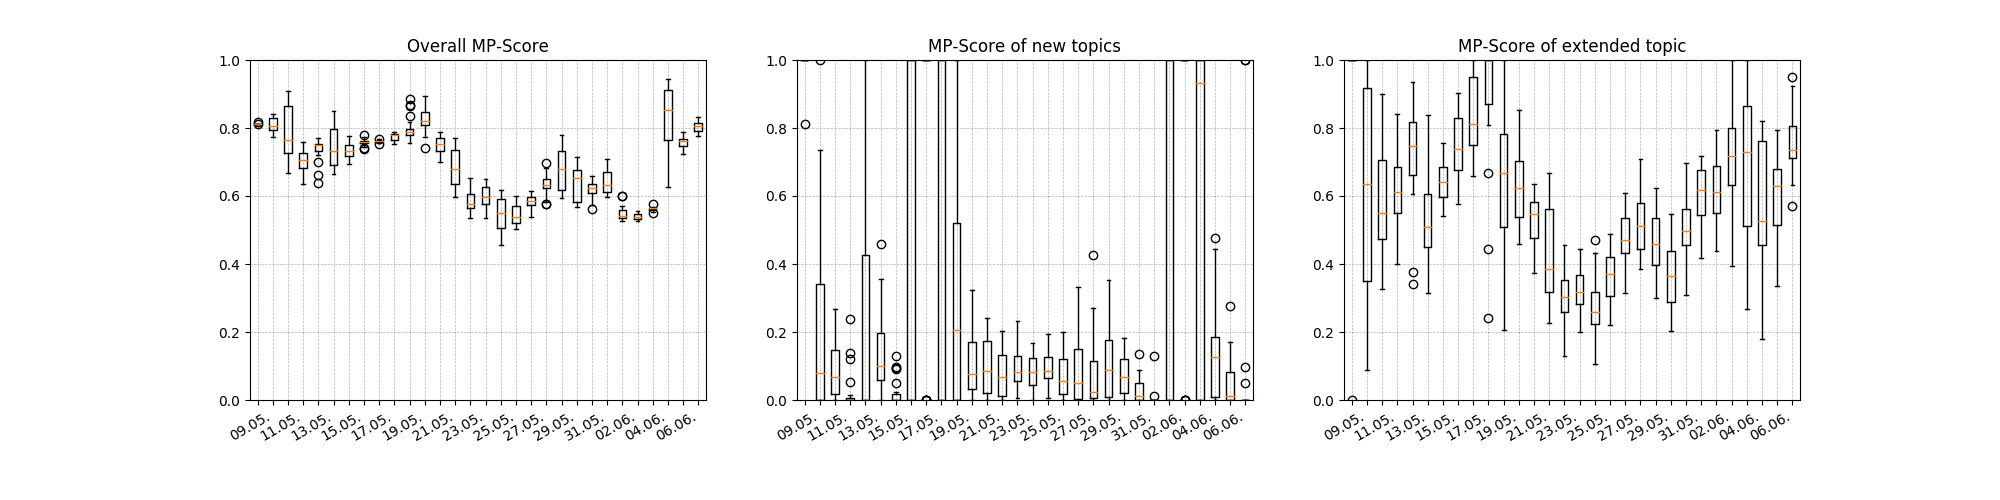
\includegraphics[width=1\textwidth]{event_detection_mp_score_1000}
    \caption{MP-Scores for clusterings using batch size of 1000}
    \label{fig:event_detection_mp_score_1000}
\end{figure}

Looking at an increased batch size of 5000 in Figure \ref{fig:event_detection_mp_score_5000}, we note that there is less variance in the overall MP-Score, which compares the full clustering with the ground truth. Although the variance for new and existing event detections is still fairly high. Additionally while the variance is high, the median for new topics is mostly around 0.1. This tells us that most of the newly detected events do not correspond with new events according to the ground truth. The detection of extensions of existing events is generally more accurate with a median between 0.5 and 0.8 using n=5000, but there is still are wide variance noticeable.  

\begin{figure}[h]
    \centering
    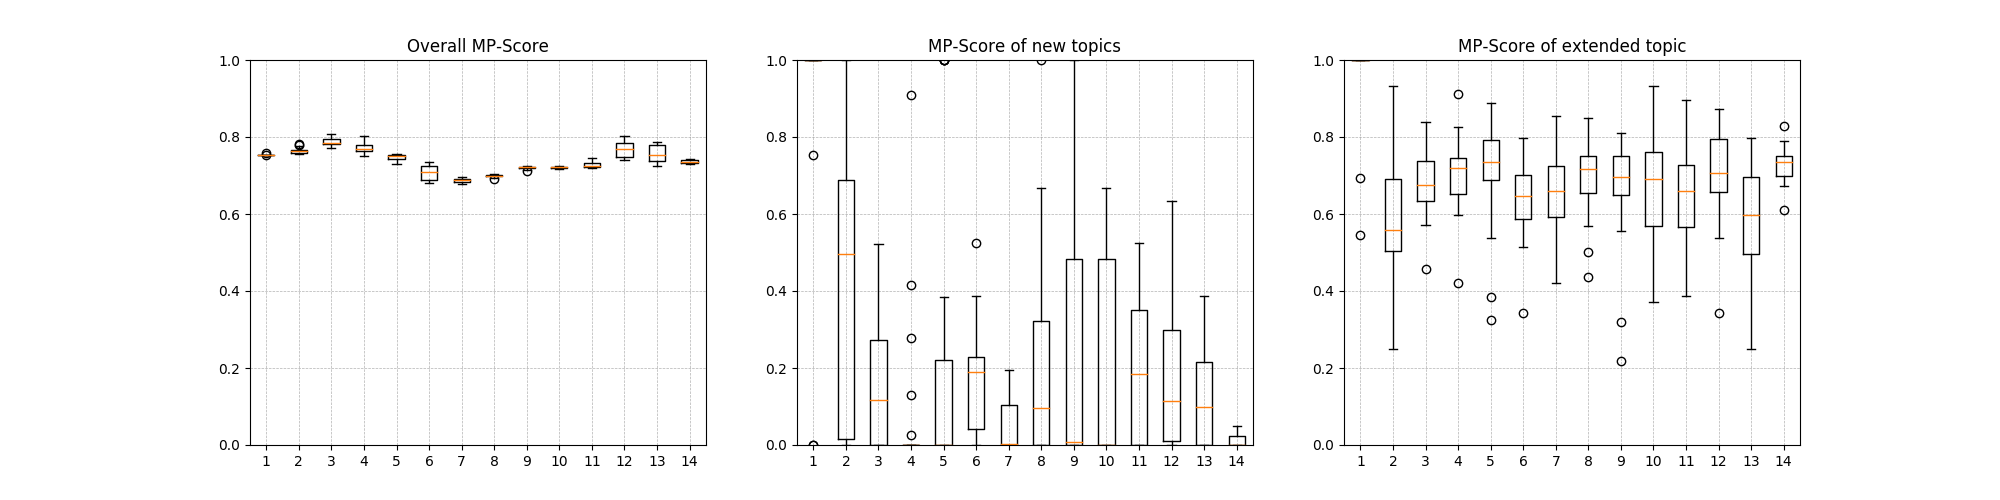
\includegraphics[width=1\textwidth]{event_detection_mp_score_5000}
    \caption{MP-Scores for clusterings using batch size of 5000}
    \label{fig:event_detection_mp_score_5000}
\end{figure}

One of the reasons for the difference in the accuracy of the detection of new events and the extension of events can be explained by the $min\_cluster\_size$. In the current setting the $min\_cluster\_size$ is set to 5, which means if an event occurs in batch one containing only four news articles, it will be discarded as noise. If the second batch contains additional news articles for the same event, it will be detected as a new occurrences, but the ground truth treats it as an existing event. To see how this affects the result we run the same simulation with a batch size of n=3000 a second time, but only considering new events from the ground truth if the number of news articles.

TODO new figure

Additional reasons for the general low performance might be due to the noise rate and the difference in the number of news articles. As described in the section about the cluster method evaluation, the noise rate for sample sizes between 1000 and 5000 ranges from 20\% to 30\%. This means a significant amount gets discarded as noise and thus potential new events might not even be detected, because too many of their news articles are discarded. Once an event is detected, detection in changes are more reliable than for new events, but as the variance in the MP-Score shows, there is still a fairly large error rate. The difference in the number of news articles in the overall clustering compared to the total number of news articles, which are part of an event in a single batch.      

As a final note let us look at two specific examples. One where the detection was mostly accurate and a second where the detection failed.

TODO 

\subsubsection{Conclusion}

While the overall clustering results in good scores, the detection of new events and changes in existing events gives rather poor results. Possible reasons have been explored such as the $min\_cluster\_size$, the noise rate or the general difference in the number of news articles, but there exist no simple solutions for any of them. As a result we conclude that the accuracy of the clustering method used in this approach is insufficient for the detection of events in a news stream.    

% TODO elaborate a bit more
\section{Conclusion}
\label{sec:6_conclusion}

\subsection{Summary}
\label{subsec:6_summary}

We started our work by searching for a suitable data set to create our clustering evaluations with.
The primary requirement was to have data points with corresponding cluster labels.
Having a labelled data set allows us to apply external measures
and evaluate a resulting clustering against the ground truth.
After selecting a few data set for closer inspection, we settled on the News Aggregator Data Set,
which contains 422,937 labelled news articles, where a label describes the story the news article is about.
Since the same story label applies to multiple news articles, we could use this as a cluster descriptor.
Unfortunately the data set only contained headlines, which did not contain enough information for our approach.
Therefore we collected the full text from each news article based on the provided source url.
The content retrieval process turned out to generate a significant amount of noise,
due to expired urls, paywalls, parsing errors or wrong redirects.
To reduce the noise, we applied different cleansing techniques
and ended up with 235,070 usable news articles.

Once the data set was ready, we designed an evaluation framework to automatically run clustering methods
with a variety of settings.
The focus was to find a combination of text preprocessing methods,
vector space model and parameters for the clustering method, which would provide the best clustering.
Furthermore we developed a custom scoring function to measure the results of a clustering,
since existing measures proved to be unintuitive and biased against certain results,
such as the number of clusters.
The analysis gave valuable insight into the behaviour of HDBSCAN with different vector space models
combined with different preprocessing methods and parameters.
We noted the initial good performance and the decrease in the quality of the clustering the larger sample sets.
However the amount of news articles proved to be substantial with up to 30\%.
Possible explanations were explored,
such as actual noisy data and different representations of articles belonging to the same cluster with tf-idf.
Furthermore we found HDBSCAN to be both faster and more precise than \textit{k}-means.

Having determined the optimal settings in the HDBSCAN evaluation,
we applied them for the event detection using a simulated stream of news articles.
The event detection was accomplished by running the clustering in batches over time.
We explored three methods for setting the batch size and different similarity thresholds for finding pairs of clusters between batches.
Since finding pairs of clusters, requires a large enough overlap in identical news articles,
the batch size has to account for this factor with regards to the volume of incoming news articles
through the data stream. 
The best method for determining the batch size turned out to be based on a fixed time period,
where we load samples from the past 24 hours for every batch. 
Thus peaks in volume during this time period will be included and not cut off by a static batch size.  
Additionally since events are represented as clusters,
the sum of events can be regarded as a subclustering of the overall clustering.
Although this makes the subclustering more sensitive to the noise rate, due to the smaller size of events.
In conclusion we found the precision of the event detection to have a high variance for new events, 
rendering it rather unstable in its current form.
A continuation of this work should focus on improving the overall clustering to increase the precision of the event detection.

\subsection{Future Work}
\label{subsec:6_future_work}

The approach in its current state still leaves different areas up for improvement.
Further work on \Gls{ner}, might help in drastically reducing the dimensionality of the vector space model
and condense a news article into only a few key entities.
Using a pretrained model did not result in accurate results,
but training a model specifically on a new corpus might improve the \Gls{ner} significantly.
Another preprocessing technique, which we did not look at, would be word embeddings.
Word embeddings allow for the detection of similar words and therefore reduce the dimensionality
of the vector space model substantially more than even Text Lemmatization.
Thus leading to a potential improved clustering and reducing the noise rate.

During our evaluation we did not explore using a dynamic time interval for running the batchwise online clustering. 
One example could be instead of using a fixed interval of one hour, a clustering would start as soon enough news articles have been collected.
Although we do not assume any considerably improvements in the precision of the event detection, 
since it would still be affected by the high noise rate. Nonetheless once the issue with the noise rate has been solved, 
this might be an interesting alternative to the dynamic batch sizes.

As we have shown, the current implementation of HDBSCAN
still leaves room for improvement in regards to space complexity.
Finding potential optimizations in memory consumption would not necessarily improve our approach,
since the quality of clusters decreases with larger sample sets,
but might be a valuable contribution to the community and enable future work with larger data sets.

We focused mainly on HDBSCAN in our analysis, but the evaluation framework allows for many different clustering methods.
Finding different methods suitable for text clustering
or even a combination of different algorithms might lead to better results.
Although we did try out some different variations such as HDBSCAN with LDA,
but without any notable results.

Furthermore it would be interesting to see how HDBSCAN would perform
using a data set based on a different kind of textual data.
A possible alternative data set could be based on computer logs,
which would also provide a source for data streams.
Improvements in the overall performance of HDBSCAN will also significantly improve the event detection in data streams.

\subsection{Lessons Learned}
\label{subsec:6_lessons_learned}

% State the 3 biggest lessons learned.
% E.g. HDBSCAN is slightly better than sklearn but way faster.

We learned that HDBSCAN is quite a versatile and efficient clustering algorithm
and at the same time experienced the challenges in text mining. 
The wide variety in types of articles and the noisy data caused the noise rate to be quite high.
We underestimated at the beginning the effect this would have on the quality of the clustering 
and moreover on the precision of the event detection.

Another lesson we learned was the importance of understanding and exploring the scoring function in more detail.
We did not research the scoring function we used in the beginning enough to be aware of their biases.
As a result we had to restart our evaluations, once we found these anomalies in our results and 
ultimately developed our own function.  

Further we learned to question our third-party libraries even well established ones such as scikit-learn.
While researching the theory for tf-idf, we could not reproduce the results produced by scikit-learns tf-idf.
It turned out scikit-learn uses a slightly different formula from the official theory. 
Additionally the implementation of HDBSCAN is not optimized for memory consumption, 
which we found out by looking through the issues on github. 

\section{Index}

% 6.1 Literaturverzeichnis
\subsection{Bibliography}
\renewcommand*{\UrlFont}{\rmfamily}
\printbibliography[heading=none]

% 6.2 Glossar

% Remove glossary title.
\renewcommand{\glossarysection}[2][]{}

% Add glossary entries.
\newglossaryentry{Vectorizer}
{
    name=vectorizer,
    description={A vectorizer transform a text into a numeric vector}
}
\newglossaryentry{Clustering}
{
    name=clustering,
    description={The task of grouping a set of objects based on their similarity}
}
\newglossaryentry{Docker}
{
    name=docker,
    description={A tool to package the application with all its dependencies as a single deployable unit and run it on independently from the underlying host}
}
\newglossaryentry{Dockerized}
{
    name=dockerized,
    description={An application environment running as a single or a collection of docker containers}
}
\newglossaryentry{API}
{
    name=api,
    description={An application programming interface allowing access to data or features of an application}
}

% Print glossary.
\glsaddall
\subsection{Glossary}
\printglossaries

% 6.3 Abbildungsverzeichnis

% Remove the list of figures title.
\makeatletter
\renewcommand\listoffigures{%
        \@starttoc{lof}%
}
\makeatother

% Print the list of figures.
\subsection{List of Figures}
\label{subsec:7c_list_of_figures}

\listoffigures

% 6.4 Tabellenverzeichnis

% Remove the list of tables title.
\makeatletter
\renewcommand\listoftables{%
        \@starttoc{lot}%
}
\makeatother

% Print the list of tables.
\subsection{List of Tables}
\listoftables

% 6.5 Symbolverzeichnis

\opensymdef
\newsym[Menge aller natuerlichen Zahlen ohne die Null]{symnz}{\mathbb{N}}
\newsym[Menge aller natuerlichen Zahlen einschliesslich Null]{symnzmn}{\mathbb{N}_{0}}
\newsym[Menge aller ganzen Zahlen]{GZ}{\mathbb{Z}}
\newsym[Menge aller rationalen Zahlen]{RatZ}{\mathbb{Q}}
\newsym[Menge aller reellen Zahlen]{RZ}{\mathbb{R}}
\newsym[Aufrechter Buchstabe]{AB}{\text{A}}
\closesymdef

\listofsymbols

% 6.6 Abkürzungsverzeichnis
\glsaddall
\subsection{List of Abbreviations}
\printglossary[type=\acronymtype]

% 6.7 Stichwortverzeichnis


\section{Appendix}
\label{sec:8_appendix}

\subsection{Algorithm for the MP-Score}
\label{subsec:8_algorithm_for_the_mp_score}

\begin{lstlisting}[language=Python, caption=Calculate the MP-Score between two clusterings., label={lst:select_max_values}]
import collections


def calculate_mp_score(true_clusters, predicted_clusters):
    """
    Calculate the mp_score of a clustering based on the contents of the clusters and the overall difference in
    predicted over true number of clusters. The calculation is based on three steps:
        1. Create an similarity matrix by calculating the difference between each cluster of both clusterings.
        2. Select the most relevant values from the similarity matrix and make sure no two clusters are being used 
           at the same time.
        3. Calculate the weighted average, where the weight is based on the true and predicted amount of elements 
           in a cluster.
    
    Parameters
    ----------
    true_clusters: array[clusters]
        2-dimensional array of true clusters
    
    predicted_clusters: array[clusters] 
        2-dimensional array of predicted clusters
    """

    # If both clusters are empty, they are identical.
    if len(true_clusters) == 0 and len(predicted_clusters) == 0:
        return 1

    similarity_matrix = create_similarity_matrix(true_clusters, predicted_clusters)
    unique_indices = select_max_values(similarity_matrix)
    return calculate_weighted_average(unique_indices, true_clusters, predicted_clusters)


def create_similarity_matrix(true_clusters, predicted_clusters):
    similarity_matrix = []
    for true_cluster in true_clusters:
        true_set = set(true_cluster)
        n_true = float(len(true_set))
        row = []
        for predicted_cluster in predicted_clusters:
            cluster_set = set(predicted_cluster)

            # Calculate the similarity using the jaccard index
            similarity = len(true_set.intersection(cluster_set)) / len(
                true_set.union(cluster_set)
            )
            row.append(similarity)

        similarity_matrix.append(row)
    return similarity_matrix


def select_max_values(precision_matrix):
    unique_indices = dict()
    row_index = 0
    nrows = len(precision_matrix)

    while row_index < nrows:
        ignore_indices = set()
        max_value_found = False

        while not max_value_found:
            max_value = 0
            column = 0
            for col_index, value in enumerate(precision_matrix[row_index]):
                if value >= max_value and col_index not in ignore_indices:
                    max_value = value
                    column = col_index

            if (
                max_value > 0
                and column in unique_indices
                and unique_indices[column]["row_index"] != row_index
                and unique_indices[column]["max_value"] > 0
            ):
                if unique_indices[column]["max_value"] < max_value:
                    # The column is already used, but we found a better
                    # candidate. We use the new candidate and set the
                    # cursor to the old one to find a new max value.
                    old_row_index = unique_indices[column]["row_index"]
                    unique_indices[column]["row_index"] = row_index
                    row_index = old_row_index
                    unique_indices[column]["max_value"] = max_value
                    max_value_found = True
                else:
                    # The column is already used by a better candidate.
                    ignore_indices.add(column)
            else:
                # If max_value is greater than 0, we store the value as a
                # new candidate. Otherwise either the row does not match
                # any other column or the max_value was low and got
                # overridden by previous tries and no other match is available.
                if max_value > 0:
                    # The column is free to use
                    unique_indices[column] = {
                        "row_index": row_index,
                        "max_value": max_value,
                    }
                max_value_found = True
                row_index += 1

    return unique_indices


def calculate_weighted_average(unique_indices, true_clusters, predicted_clusters):
    mp_score = 0

    elements_per_true_cluster = [len(cluster) for cluster in true_clusters]
    elements_per_predicted_cluster = [len(cluster) for cluster in predicted_clusters]

    total_true_elements = sum(elements_per_true_cluster)
    total_pred_elements = sum(elements_per_predicted_cluster)
    total_elements = total_true_elements + total_pred_elements

    if total_elements > 0:
        for column, value in unique_indices.items():
            # The row of the similarity matrix equals the index of the true cluster, while the column is the index of the predicted cluster
            weight = (
                elements_per_true_cluster[value["row_index"]]
                + elements_per_predicted_cluster[column]
            ) / (total_elements)
            mp_score += value["max_value"] * weight

    return mp_score
\end{lstlisting}


\end{document}
